\chapter{Приложения моделей близости ключевых слов} \label{chapt_applications}
% SYNOPSIS_4 >>>
В настоящей главе рассматриваются решения востребованных на практике задач, необходимые для этого модели и алгоритмы, их программные реализации.
Представляется авторское решение задачи кластеризации ключевых слов информационной системы. Рассматривается задача поиска экспертов в области, определяемой запросом из заданного набора ключевых слов.  Приводится решение задачи определения тематики объекта информационно-аналитической системы. Описывается также процедура использования тезауруса ключевых слов для решения задачи улучшения результатов ранжирования в поисковой составляющей информационно-аналитической системы <<ИСТИНА>>.  В заключении главы представлены выводы, а также дальнейшие направления применения разработанных автором программных средств в приложениях, которые диктуются практикой использования большой наукометической системы.
% <<< SYNOPSIS_4

\section{Модель семантической кластеризации ключевых слов} \label{clustering}
Механизмы кластеризация ключевых слов любой большой информационно-аналитической системы являются важным аналитическим инструментарием анализа данный. В первую очередь, они важны для систем, не обладающих необходимыми для получения надежного результата объемами данных. В таких системах, как правило, нет достаточного количества информации о ее объектах и о соответствующих этим объектам ключевых словах. Как следствие,  значительная доля ключевых слов будет иметь низкие частоты встречаемости в системе, что делает затруднительным любые аналитические процедуры для таких слов. Преодолеть эти трудности можно путем решения задачи кластеризации. При таком подходе появляется возможность разбить все множество ключевых слов на кластера из семантически близких слов. После подобной предобработки можно отождествить исходные слова с соответствующими им кластерами, что предоставит более богатую статистику встречаемости для каждого ключевого слова.

В настоящем разделе описывается разработанный автором подход к решению данной задачи. В первых подразделах описывается новая модель кластеризации ключевых слов информационно-аналитической системы, основанная на мере \emph{контекстной близости}, которая была введена в \ref{cont_sim}. С помощью такой меры конструируется граф, именуемый далее \emph{контекстным графом}. После этого используются  дополнительные эвристические соображения, позволяющие отбросить наименее значимые связи в этом графе. Такой граф получил название \emph{усеченный контекстный граф}. Далее описывается метод кластеризации этого грава.  Заключительная часть раздела посвящена опробации программной реализации разработанной модели и выводам.

Задача кластеризации формулируется следующим образом. Задано множество ключевых слов рассматриваемой системы $W = {w_1, \cdots, w_N}$. Необходимо построить такое отображение $c: W \rightarrow \mathbb{N}$, ставящее в соответствие каждому ключевому слову системы номер кластера, которому это слово принадлежит. Условие, которое накладывается на эту функцию $c$, заключается в том, что все слова, попавшие в один кластер, должны быть семантически близкими понятиями, а слова из разных кластеров должны семантически различаться.

%\subsection{Модель построения полного и усеченного контекстных графов ключевых слов} \label{trunc_cont}
\subsection{Модель полного контекстного графа ключевых слов} \label{full_cont}
Ненулевое значение введенной в разделе \ref{cont_sim} величины $C_{T}(w_i,w_j)$ означает контекстную связь между ключевыми словами. На основе контекстной близости естественным выглядит построение графа, вершинами которого являются ключевые слова коллекции $T$. Ребро между парами вершин обозначается в случае, если соответсвующая пара имеет ненулевой уровень контекстной близости. Обозначим данный граф за $G_{cont}$. Таким образом, модель данных, лежащая в основе исследуемого подхода к кластеризации ключевых слов, является графовой моделью. Ключевые слова хранятся в вершинах, а для определения факта существования ребра используется модель контекстной близости, описанная в \ref{cont_sim}. Представляется целесообразным использовать данный граф для решения поставленной задачи кластеризации ключевых слов. Однако сразу отметим, что такой граф имеет ряд недостатков.

Несмотря на то, что для значительной части пар ключевых слов значение $C_{T}(w_i, w_j)$ равно нулю, существует большое число ненулевых связей, что затрудняет их дальнейший анализ с технической точки зрения. Каждая вершина в графе может быть связана с тысячами других вершин. Это обстоятельство значительно увеличивает вычислительную нагрузку на любые используемые графовые алгоритмы.

В дополнении к изложенному выше, низкие значения контекстной близости пары слов зачастую являются ненадежными. Если значение контекстной близости мало, то этот факт означает, что у пары слов мало общих соседей в графе ключевых слов и связь с этими общими соседями имеет небольшой вес. Низкие ненулевые значения контекстной близости могут иметь даже семантически различные пары, поскольку связь в этом случае не является статистически надежной. Такие данные не привносят полезной информации, а только ухудшают качество работы реализованных алгоритмов.

По изложенным причинам возникает необходимость в усечении графа, собранного согласно описанной выше модели. Под усечением понимается удаление ребер, которые представляют наименее качественные и статистически проверенные связи. Описание модели усеченного контекстного графа приводится в следующем далее подразделе.

\subsection{Модель и алгоритм построения усеченного контекстного графа ключевых слов} \label{trunc_cont}

В качестве модели данных усеченного контекстного графа принята модель, схожая с введенной в предыдущем подразделе моделью $G_{cont}$. Основное отличие новой модели состоит в более сильных условиях, определяющих факт существования ребра между парой вершин, что ведет к значительно меньшему числу ребер в графе. Эти условия нацелены на удаление семантически незначащих ребер из графа $G_{cont}$.
    
Автором определены следующие эвристические cоображения, определяющие модель усеченного контекстного графа.
\begin{enumerate}
    \item \textbf{Для всех ключевых слов $w_i$ фильтруются связи со слишком низким уровнем близости $C_{T}(w_i,w_j)$.}

    Этот шаг необходим для того, чтобы удалить слабые связи и ненадежные связи из рассмотрения и оставить только наилучшие. Следует также отметить, что одного этого соображения недостаточно для качественного удаления лишних ребер. Причиной этому является тот факт, что сами значения близости $C(w_i,w_j)$ не так важны, как порядок, который они задают на множестве соседей вершины $w_i$.  Другими словами, данная задачу фильтрации стоит рассматривать как задачу ранжирования соседей вершины $i$ , а не как задачу классификации ребер $(w_i, w_j)$ на классы полезных и бесполезных ребер.
    \item \textbf{От оставшихся выбирается некоторая доля связей (например, 20\%) с наибольшими значениями $C_{T}(w_i,w_j)$ .}

    Такое условие представляется естественным, потому что слова, которые встречаются со многими другими в одинаковых контекстах, должны иметь больше ребер в графе, чем те слова, которые контекстно близки только с небольшим числом слов.

    \item \textbf{Количество отобранных связей должно находиться в некоторых рамках (например, не менее 3 и не более 10 соседей на вершину).}

    Верхняя граница является преимущественно техническим ограничением: если было взято 20\% от числа всех соседей, но это число оставшихся связей по-прежнему достаточно велико, то хранение таких вершин потребует значительных ресурсов. Нижняя граница берется для того, чтобы вершина, для которой имеется мало кандидатов, получила хотя бы их в качестве ребер. С учетом ограничения из п.1. можно ожидать, что эти связи будут достаточно качественными для дальнейшего анализа.

    \item \textbf{Общее количество оставшихся связей должно быть ограничено сверху (например, не более 1000000 ребер в графе)}

    Слишком большое число ребер в графе негативно сказывается на вычислительной производительности системы. В то же время, сильное ограничение на максимальное количество ребер  не позволяет модели использовать в полной мере полезный сигнал из подлежащих анализу данных.

\end{enumerate}

Граф, ребра которого отфильтрованы по указанным выше правилам, обозначим за $G_{cont\_trunc}$ и назовем \emph{усеченным контекстным графом}. Далее приведено более формальное описание алгоритма, реализующего введенную выше модель.

\begin{itemize}
    \item Входные параметры:
        \begin{itemize}
            \item пороговое значение $C_{thr}$;
            \item минимальное и максимальное число ребер для одной вершины в усеченном графе $n_{min}, n_{max}$;
            \item максимальная доля ребер вершины, которая переносится из графа $G_{cont}$ в граф $G_{cont\_trunc}$ - $ratio$;
            \item максимальная число ребер в графе $G_{cont\_trunc}$ - $n_{edge\_max}$.
        \end{itemize}
    \item Удаляются все ребра $(w_i, w_j)$, для которых значение $C_{T}(w_i, w_j) < C_{thr}$.
    \item Пусть $rank_j$ - порядковый номер соседа $w_j$ в отстортированном по убыванию значения $C_{T}(w_i,w_j)$ списке всех соседей вершины $w_i$. Тогда, если $rank_j > \max(n_{min},\min(n_{max},n * ratio))$, то связь $(w_i,w_j)$ должна быть отфильтрована. Здесь $n$- число соседей вершины $w_i$ в полном контекстном графе.
    \item Если число ребер, оставшихся в результате фильтрации, превышает $n_{edge\_max}$, то выбирается выбирается $n_{edge\_max}$ ребер $(w_i, w_j)$ с наибольшими значениями $C_T(w_i, w_j)$.
\end{itemize}

Можно отметить, что в описанном выше алгоритме присутствует значительное число параметров, а именно - $C_{thr}, n_{min}, n_{max}, ratio, n_{edge\_max}$. Значение входных параметром преимущественно зависят от специфики исследуемой системы, а также от объема входных данных. Несмотря на это, выбор конкретных значений не является сложной задачей, покольку значения параметров $n_{min}, n_{max}, ratio$ слабо варьируются в зависимости от входных данных. Для построения графа в программной реализацией алгоритма были использованы входные значения параметров $n_{min} = 3, n_{max} = 10, ratio=0.2$. Отмачается, что данные значения являются адекватным приближением для этих параметров и могут быть использованы при внедрении в другие, отличные от используемой в эксперименте интеллектуальные системы. Значение параметра $n_{edge\_max}$ зависит от объема вычислительных ресурсов, имеющихся на поддержание работоспособности системы. 

Единственным параметром, требующим дополнительного анализа, является параметр $C_{thr}$. Причиной является тот факт, что введенная ранее контекстная мера близости не устойчива к изменению входных данных. Это означает, что для разных коллекций ключевых слов $T$ и $T'$ оказываются разными значения контекстной блиости $C_T(w_i, w_j)$ и $C_T'(w_i, w_j)$. Более того, значения, при которых с высокой долей вероятности можно заключать сильную семантическую связь между парой ключевых слов в разных коллекциях ключевых слова могут значительно разниться. 

Для определения оптимальных значений параметров автором разработан описанный далее в разделе \ref{clustering_test} метод, преимущество которого состоит в полной автоматизации процесса настройки. 

Отмечается также, что ребра построенного графа могут быть помечены числами и представляется возможным ввести функцию расстояния между вершинами. Например, такой функцией может служить величина $C_{T}(w_i,w_j)$. В рамках рассматриваемого подхода, ребра графа остаются непомеченными, что существенно понижает сложность и не ухудшает качество разработанных моделей.

В следующих далее подразделах описывается процедура кластеризации построенного усеченного графа $G_{cond_trunc}$. Реализация этого алгоритма демонстрирует высокий уровень качества в тестовых испытаниях. В большинстве случаев выделенные кластера ключевых слов состоят из попарно близких по смыслу ключевых слов. Данный факт подтверждеются тестовыми испытаниями, описанию которых посвящен подраздел \ref{clustering_test}.

\subsection{Модель кластеризации усеченного контекстного графа} \label{clustering_procedure}
Ребра усеченного контекстного графа, который был введен в предыдущем подразделе, в большей мере показывают семантическую близость между парой вершин, чем ребра полного контекстного графа и, тем более, графа ключевых слов. При этом отметим, что усеченный граф значительно уменьшает вычислительные затраты. Он повышает точность выявленных семантических связей между ключевыми словами. По этой причине рассмотрение длинных путей в графе становится более оправданным, поскольку семантическая близость между парой вершин лучше сохраняется с увеличением расстояния в графе.  Поясним данное утверждение на следующем примере.

Предположим, что заданы 2 графа: полный контекстный граф $G_{cont}$ и усеченный контекстный граф $G_{cont\_trunc}$. Для ясности допустим, что пара слов либо является семантически близкой, либо таковой не является. Другими словами, уберем все возможные <<градации>> семантической близости и не будем рассматривать случаи, когда пара слов \emph{сильно} или \emph{слабо} связана по смыслу.
    
Далее предположим, что ребро в графе с некоторой вероятностью отражает факт семантической близости между соответствующими вершинами. Обозначим эти вероятности за $p_{cont}$ и $p_{cont\_trunc}$ для графов $G_{cont}$, $G_{cont\_trunc}$. По построению очевидно, что $p_{cont\_trunc} > p_{cont} $, поскольку из графа $G_{cont\_trunc}$ исключены те ребра, которые с меньшей долей уверенности соединяют семантически близкие ключевые слова.

Далее рассмотрим тройку ключевых слов $w_i, w_j, w_k$ графа $G_{cont}$ таких, что в графе присутствуют ребра $(v_{w_i}, v_{w_j})$ и $(v_{w_j}, v_{w_k})$, но отсутствует ребро $(v_{w_i}, v_{w_k})$. Необходимость кластеризации заключается в том, что по имеющимся семантическим связям появляется возможность восстановить отсутствующие связи. Такие отсутствующие связи имеет место быть, например, по причине недостатка исходных данных.

Допустим, что некоторый алгоритм кластеризации отнес слова $w_i, w_j, w_k$ в один и тот же кластер. Это факт означает, что появилась гипотеза о семантической близости ключевых слов $w_i, w_k$, которой не было изначально. Исходя из определения введенной модели, можно оценить вероятность того, это действительно пара семантически близких слов. С вероятностью $p_{cont}$ семантически близки слова $w_i$ и $w_j$, с той же вероятностью семантически близкими являются слова $w_j$ и $w_k$. Тогда вероятность близости пары ключевых слов $w_i$ и $w_k$ можно определить как $p_{cont}^2$, предположив транзитивность отношения семантической близости в рамках данной модели. Другими словами, для того, чтобы $w_i$ и $w_k$ были семантически близки, достаточно, чтобы были семантически близки и слова пары $(w_i, w_j)$, и слова пары $(w_j, w_k)$. Вероятность одновременного выполнения этих условий равна $p_{cont}^2$.  %Кроме того, ключевые слова $w_i$ и $w_k$ могут быть соединены через другие вершины в графе, но данное обстоятельство не рассматривается в рамках данной модели. 

Аналогично можно показать, что если в графе существует путь между вершинами $w_i, w_k$ длины $n$, то есть существует последовательность ребер $(v_{w_i}, v_1), (v_1, v_2), \cdots, (v_{n-3}, v_{n-2}), (v_{n-2}, v_{w_k}) $, то при отсутствии других путей вероятность семантической близости пары $(w_i, w_k)$ равна $p_{cont}^n$. Таким образом, с увеличением расстояния между словами в графе, вероятность семантической близости экспоненциально уменьшается.

Теперь заметим, что все описанные выше рассуждения в той же мере верны для графа $G_{cont\_trunc}$. Однако, в связи с тем, что $p_{cont\_trunc} > p_{cont}$, то скорость убывания вероятности семантической близости с увеличением расстояния в графе будет ниже в графе $G_{cont\_trunc}$. При этом, если значение $p_{cont\_trunc}$ близко к 1, то вероятность семантической близости для вершин, расположенных на расстоянии, например, 3 или 4, в графе будет достаточно высокой. Отмечается, чем больше ребер было удалено при построении графа $G_{cont\_trunc}$, тем сильнее оценка уровня семантической связи между вершинами, ребра которых прошли фильтрацию, и тем больше значение вероятности $p_{cont\_trunc}$. 

Следует однако отметить тот факт, что для пары слов $(w_i, w_k)$ в любом из графов может присутствовать множество различных путей. Наличие большего числа путей, очевидно, должно положительно отражаться на вероятности того, что ключевые слова $(w_i, w_k)$ являются семантически похожими. Кроме того, заметим, что по построению графа $G_{cont\_trunc}$, между любой парой вершин в этом графе \emph{не больше} различных путей, чем в графе $G_{cont}$.

Данное замечание приводит к следующим двум возможным стратегиям поиска неявных семантических связей:
\begin{enumerate}
    \item использование большого числа коротких путей в графе $G_{cont}$; 
    \item использование небольшого числа длинных путей в графе $G_{cont\_trunc}$. 
\end{enumerate}

Фактически, коротким путем для графа $G_{cont}$ можно считать путь длины 2, а длинным путем для $G_{cont\_trunc}$ пути, длины 3 и более.

Использование графа $G_{cont\_trunc}$ имеет неоспоримое преимущество. Оно заключается в возможности гибкой настройки структуры этого графа посредством параметров алгоритма построения усеченного контекстного графа. Таким образом, данный факт делает возможным \emph{компромиссную стратегию выявления неявных связей}:
\begin{itemize} 
    \item чем больше ребер осталось в графе $G_{cont\_trunc}$, тем меньше необходимо использовать длинные пути и тем большее число коротких путей, доступных для анализа;
    \item чем меньше ребер осталось в графе $G_{cont\_trunc}$, тем больше возможность использования длинных путей, но тем меньше их число.
\end{itemize}

При этом следует отметить, что преимущество графовых подходов к задаче кластеризации состоит в возможности учитывать длинные пути в процессе построения кластеров. По этой причине в основе предложенного автором метода кластеризации лежит известный графовый алгоритм кластеризации, прошедший опробацию в различных практических задачах.

В следующем далее подразделе описывается алгоритм кластеризации, разработанный в рамках представленной модели.

%Вследствии этого возникает задача кластеризации графа: разделение множества всех вершин на подмножества таким образом, что любая пара вершин из одного множества является парой близких по смыслу ключевых слов.
\subsection{Алгоритм кластеризации усеченного контекстного графа} \label{clustering_algo}

За основу кластеризующего алгоритма, соответствующего модели из подраздела \ref{trunc_cont}, взят алгоритм Louvain Modularity \cite{louvain_modularity}. Подход, описанный в этой статье, решает задачу разбиения входного графа на кластеры таким образом, что количество ребер между вершинами одного кластера велико, а количество ребер между вершинами разных кластеров, напротив, мало. Обозначим за плотность подграфа отношение числа ребер к числу вершин этого подграфа. Тогда в рамках данной задачи необходимо максимизировать плотность внутри внутри одного кластера, одновременно с этим минимизируя плотность подграфов, образованных вершинами из разных кластеров.

Качество разбиения принято измерять с помощью так называемой \emph{модулярности разбиения}. Модулярность - скалярная величина, значение которой лежит в интервале $[0, 1]$. В случае графа, ребрам которого проставлены веса, модулярность определяется следующим образом:

$$ Q = \frac{1}{2m}\sum_{i,j}[A_{ij} - \frac{k_i k_j}{2m}]\delta(c_i, c_j),$$

где $A_{ij}$ - вес ребра между вершинами $i$ и $j$, $k_i=\sum_j{A_{ij}}, m=\frac{1}{2}\sum_{i,j}A_{ij}$, $c_i$ - номер кластера, в котором лежит вершина $i$, $\delta$- дельта-функция (функция, принимающая значение 1, если $c_i=c_j$ и 0 в другом случае).

Если пара вершин $i$, $j$ принадлежат одному кластеру, то значение слагаемого в функционале для этой пары будет тем больше, чем выше ее вес и чем меньше эти вершины имеют связей с вершинами других кластеров. Вершины одного кластера, не связанные ребром друг с другом оказывают негативное влияние на значение $Q$, поскольку вес ребер в этом случае равен нулю. Если вершины располагаются в разных кластерах, то за счет дельта-функции, которая принимает нулевое значение в этом случае, явного воздействия в значение функционала $Q$ пара вершин не оказывает. Термин <<явное>> при этом означает, что соответсвующее слагаемое функционала $Q$ равно нулю. Однако отмечается, что вершины из разных кластеров уменьшают значение функциона из-за члена $\frac{k_i k_j}{2m}$ в других слагаемых.

Как показано авторами \cite{modularity_is_hard}, задача максимизации представленного выше функционала является NP-сложной, поэтому для её  решения используются аппроксимационный агломеративный алгоритм. Агломеративность означает, что при инициализации такой алгоритм создает отдельный кластер для каждой вершины, а затем объединяет кластера таким образом, чтобы максимально увеличить значение функционала $Q$. Основные шаги алгоритма описаны далее.

\begin{enumerate}
    \item Входные параметры алгоритма: взвешенный граф $G$.
    \item Для каждой вершины графа $v_i \in G$ создается свой кластер $c_i = i$.
    \item Для каждой вершины $v_i$ и для каждого соседа $v_j$ вершины $v_i$ в графе $G$ выполняется:
        \begin{enumerate}
            \item временное добавление вершины $v_i$ в кластер вершины $v_j$;
            \item подсчет изменения оптимизируемого функционала при перемещении вершины $v_i$ в кластер вершины $v_j$: $\Delta Q_{i,j}$.
        \end{enumerate}
    \item Окончательное добавление вершины $v_i$ в кластер того соседа, на котором достигается максимальное увеличение значения $Q$, то есть 
            $c_i \mathrel{{:}{=}} c_k$, где $k = \operatorname*{argmax}_j \Delta Q_{i, j}$.  Если функционал нельзя увеличить, то есть $\Delta Q_{i, j} < 0$ для всех $j$, то кластер вершины остается без изменения.
    \item Построение нового графа $G'$, вершинами которого являются кластера, а веса ребер отражают связи между кластерами. Вес ребра равен сумме весов всех пар ребер, вершины которых лежат в соответствующих кластерах.
    \item Повторение п.2-5 для графа $G'$ до полной сходимости алгоритма.
\end{enumerate}

Преимущество данного алгоритма заключается в его масштабируемости на графы больших размеров. Возможность эффективного пересчета кластеров достигается засчет быстрого пересчета изменения значения функционала качества в п.3.б представленного выше алгоритма:
$$ \Delta Q_{i,j} = \left[ \frac{\sum_{in} + k_{i,in}}{2m} - \left(\frac{\sum_{tot} + k_i}{2m}\right)^2 \right] - \left[ \frac{\sum_{in}}{2m} - \left(\frac{\sum_{tot}}{2m}\right)^2 - \left(\frac{k_i}{2m}\right)^2 \right], $$
где $\sum_{in}$ - сумма весов ребер внутри кластера вершины $v_j$, $\sum_{tot}$ - сумма весов ребер, инцидентных вершинам кластера вершины $v_j$, $k_i$ - сумма весов ребер, инцидентных вершине $v_i$, $k_{i, in}$ - сумма весов ребер, инцидентных вершине $v_i$ внутри кластера вершины $v_j$, $m$ - сумма весов всех ребер в графе. 

Следует отметить, что количество кластеров не является параметром данного алгоритма. На практике кластера, получающиеся в результате работы программной реализации алгоритма, оказываются слишком большого размера. В некоторые кластера могут попасть тысячи или десятки тысяч слов. Однако,  очевидно, что не существует такого огромного множества попарно похожих по смыслу слов. Алгоритм является общим графовым алгоритмом и никаким образом не использует информацию о семантической близости. Даже точное решение оптимизационной задачи не гарантирует качественного разбиения вершин графа на подмножества, элементы которого семантически близки друг к другу. Как следствие, необходимы дополнительные действия, связывающие процессы кластеризации графа и определения семантической близости. Далее представлен алгоритм кластеризации усеченного контекстного графа, разрешающая отмеченную трудность.

%\begin{equation}\label{}
\begin{enumerate}
    \item Входные данные алгоритма: усеченный контекстный граф $G_{cont\_trunc}$, параметр $k$ - максимальный размер кластера.
    \item Создается выходное множество кластеров $Clusters$
    \item Создается очередь $Queue$ для подграфов исходного графа.
    \item Исходный граф добавляется в нее.
    \item Пока очередь $Queue$ не пуста выполняется:
    \begin{enumerate}
        \item кластеризация подграфа, взятого из очереди, описанным ранее алгоритмом кластеризации;
        \item для каждого полученного в результате кластеризации подграфа-кластера $c$:
            \begin{enumerate}
                \item если кластер $c$ содержит меньше, чем $k$ вершин, или $c$ совпадает с кластеризуемым подграфом (не существует разбиения данного подграфа на хотя бы 2 кластера меньшего размера), то $c$ добавляется в выходное множество кластеров $Clusters$;
                \item иначе кластер $c$ добавляется в очередь подграфов.
            \end{enumerate}
    \end{enumerate}
    \item Возвращается множество определенных кластеров $Clusters$.
\end{enumerate}

Данный алгоритм позволяет проводить кластеризацию до тех пор, пока не будут получены кластеры необходимого размера. Следует отметить, что в некоторых ситуациях подграф, к которому применяется алгоритм кластеризации, может иметь размер больший, чем $k$, но быть при этом оптимальным с точки зрения максимизируемого функционала $Q$. Такой граф не может быть разделен на несколько подграфов меньшего размера, поэтому он добавляется ко множеству определенных кластеров, несмотря на свой размер. Примером такого подграфа может быть \emph{клика} (полный подграф в графе), размера большего, чем $k$.

Резюмируя представленные в данной главе соображения, автором получен алгоритм кластеризации ключевых слов коллекции $T$, описание которого следует далее.  
\begin{itemize}
    \item Для ключевых слов коллекции $T$ вычисляется степень контекстной близости.
    \item Выполняется построение контекстного графа $G_{cont}$.
    \item Для графа $G_{cont}$ выполняется процедура построения усеченного контекстного графа $G_{cont\_trunc}$.
    \item С помощью алгоритма кластеризации усеченного контекстного графа, вычисляются необходимые кластеры ключевых слов коллекции.
\end{itemize}

Таким образом, автором разработан алгоритм кластеризации ключевых слов по входной коллекции $T$. Данный алгоритм получил название \emph{ContGraphClustering}. Эффективность реализации данного алгоритма, а также качество производимой им кластеризации ключевых слов обосновываются в следующем далее подразделе $\ref{clustering_test}$.
\subsection{Тестовые испытания} \label{clustering_test}

Описанный ранее алгоритм кластеризации контекстного графа позволяет удалять недостаточно надежные связи между словами, полученные с помощью алгоритма определения близости по контекстному графу, и, наоборот, добавлять новые ребра между семантически похожими парами слов. 

Рассмотрим результат работы алгоритма на конкретном примере. На рисунке \ref{img:sim_2_clust} изображены несколько ближайших контекстно близких слов для слова <<студенты>>, полученных с помощью модели \emph{WordContSim}. Описание этой модели можно найти в разделе \ref{wordcontsim}. Пример со словом <<студенты>> взят из тестовых испытаний, описанных в \ref{test_sect}. Отметим, как и ранее, что полное множество соседей вершины слишком велико, чтобы его изобразить.

\begin{figure}[ht]
  \begin{minipage}[ht]{1.0\linewidth}\centering
    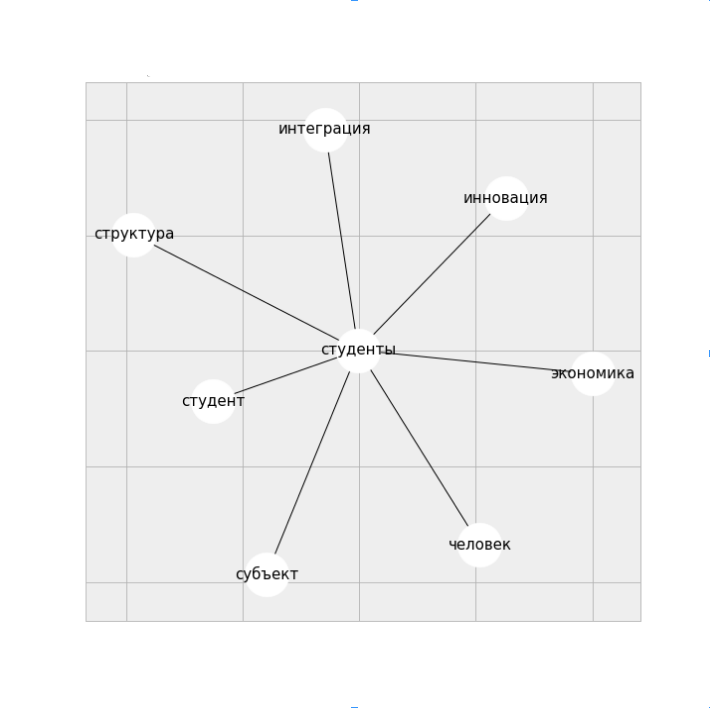
\includegraphics[width=1.0\linewidth]{Dissertation/pics/students_sim}
    \caption{наиболее близкие слова для слова <<студенты>> в контекстном графе}
    \label{img:sim_2_clust}
  \end{minipage}
\end{figure}

Кластер, полученный в ходе работы программной реализации алгоритма кластеризации для того же слова <<студенты>> изображен на рисунке \ref{img:clust_1}.

\begin{figure}[ht]
  \begin{minipage}[ht]{1.0\linewidth}\centering
    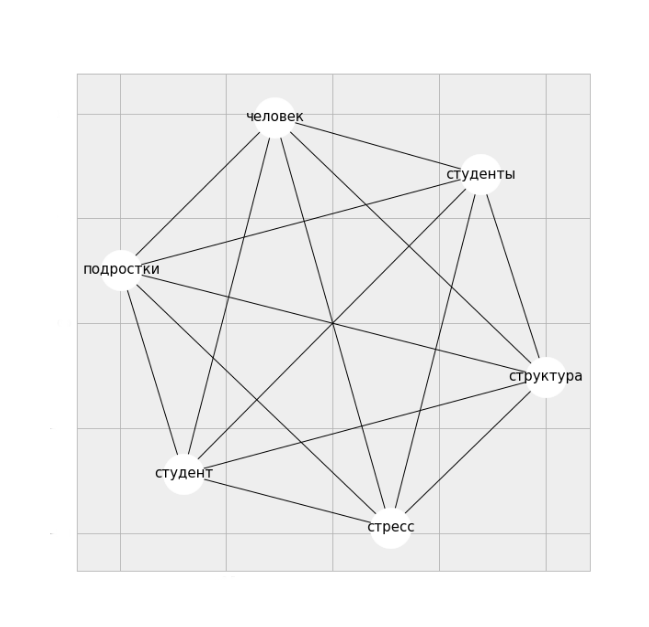
\includegraphics[width=1.0\linewidth]{Dissertation/pics/students_cluster}
    \caption{кластер, содержащий слово <<студенты>>}
    \label{img:clust_1}
  \end{minipage}
\end{figure}

Можно заметить, как в результате кластеризации были разорваны связи (т.е. удалены ребра в графе) <<студенты-экономика>>,  <<студенты-инновации>>, вместо которых на первый план вышли связи <<студенты-подростки>>. Отмечается также, что выбранный метод кластеризации графа может допускать ошибки. Например, в случае с парой <<студенты-структура>>, которая была как в усеченном контекстном графе, так и в кластере слова студент.

Для интегральной проверки качества выбрана процедура, аналогичная описанной в разделе \ref{cont_sim_experiment}. Однако, для тестирования программной реализации алгоритма кластеризации была внесены модификации для учета специфики данной задачи. Причина ее необходимости заключается в том, что ранее алгоритм генерации тестовых примеров создавал тестовые пары ключевых слов. Однако, в рамках задачи кластеризации необходимо иметь возможность проверки реализаций алгоритмов на тестовых \emph{кластерах} - множествах семантически близких ключевых слов. 

Для достижения этой цели разработана следующая программа эксперимента. Из множества всех ключевых слов $W$ выделяется случайное множество слов $W_{test}$, на котором впоследствии будут протестированы модели. Как и ранее, последовательно просматриваются наборы $t$ коллекции $T$ и каждое ключевое слово $w \in t$. Если текущее слово является тестовым, то есть $w \in W_{test}$, то это слово заменяется на синтетически созданное слово $w^{*n*}$, где <<$*$>> - спецсимвол, а $n$ - число, взятое случайно из геометрического распределения $Geom(p)$, где $p$ - вероятность успеха в бернуллиевском эксперименте. Наличие спецсимвола в слове делает его уникальным в рамках коллекции $T$.

Таким образом, коллекция $T$ преобразуется в коллекцию $T^*$. Эта коллекция содержит для слов  $w \in W_{test}$ одно или несколько слов вида $w^{*n*}$. Это множество слов определяет один тестовый кластер. Кластер для данного слова $w$ может содержать от одного до $f_T(w)$ слов, где $f_T(w)$, как и ранее, частота встречаемости слова $w$ в коллекции. Кластеры, содержащие слишком малое количество объектов, удаляются. В программной реализации алгоритма удаляются кластеры, содержащие менее, чем 4 слова. За множество $W^*$ обозначим множество ключевых слов созданной коллекции $T^*$. Множество ключевых слов из $W^*$, попавших в тестовые кластера, обозначим $W_{clusters}$. Перенумеровав полученные тестовые кластеры, определим отображение $C_{test}: W_{clusters} \rightarrow \mathbb{N}$, которое ставит слову из $W_{clusters}$ номер его кластера.

В отличие от решения задачи определения семантической близости пар слов, данная задача не требует определения отрицательных тестовых примеров. Для тестирования достаточно указать множество тестовых кластеров. Задачей алгоритмов кластеризации в этом случае является определение такого отображения $C: W_{clusters} \rightarrow \mathbb{N}$, которое определяет кластер для каждого тестового слова. После этого с помощью метрик кластеризации определяется наиболее качественный алгоритм. Более точные алгоритмы должны построить отображение $C$ совпадающее с отображением $C_{test}$ с точностью до перенумерации кластеров. Другими словами, важно, чтобы слова из одного тестового кластера были помещены алгоритмом в один кластер, а слова из разных тестовых кластеров - в разные. Метрики, выбранные для проверки качества, описаны далее. В рамках данного подраздела будем называть кластеризацией отображение, которое ставит словам из $W_{clusters}$ номера кластеров. 
\begin{itemize}
    \item \textbf{Adjusted Rand Index (ARI).} Пусть $a$ - количество пар ключевых слов из $W_{clusters}$, которым присвоен один и тот же номер тестовой кластеризацией $C_{test}$, а также один и тот же номер испытуемым алгоритмом кластеризации $C$. 
        
        Аналогично, пусть $b$ - количество пар, слова из которых присвоены различные кластера как в $C_{test}$, так и в $C$.  
        
        Величина $RI = \frac{a + b}{C_{|W_{clusters}|}^2}$ - нескорректированная метрика $Rand Index$. Чем больше значение данной метрики, тем более правильной оказалась кластеризация, полученная испытуемым алгоритмом. Для того, чтобы значения метрики было близко к нулю в случае случайной кластеризации (кластеризации таким алгоритмом, который ставит каждому слову случайный номер кластера), вычисляется следующее скоректированное значение метрики:

        $$ARI = \frac{RI - E[\hat{RI}]}{max(\hat{RI}) - E[\hat{RI}]},$$

        где $E[\hat{RI}], max(\hat{RI})$ - математическое ожидание и максимум случайной величины $RI$, определенной алгоритмом случайной кластеризации.

    \item \textbf{V-Measure.} Для подсчета этой меры вычисляются две вспомогательные величины. 
        \begin{enumerate}
            \item Однородность (Homogeneity):
                $$ h = 1 - \frac{H(C|C_{test})}{H(C)}. $$
            \item Полнота (Completeness):
                $$ c = 1 - \frac{H(C_{test}|C)}{H(C_{test})}. $$
        \end{enumerate}

        В данных формулах используется понятие условной энтропии, которая для пары кластеризаций $C_1, C_2$ задается следующим образом:
        
        $$ H(C_1|C_2) = -\sum_{c_1=1}^{|C_1|}\sum_{c_2=1}^{|C_2|}\frac{n_{c_1, c_2}}{n}\log\left(\frac{n_{c_1, c_2}}{n_{c_2}}\right),$$

        а также понятие энтропии для кластеризации $C$, которая вычисляется по следующей формуле:

        $$ H(C)  = -\sum_{c=1}^{|C|}\frac{n_c}{n}\log\left(\frac{n_c}{n}\right).$$

        В двух последних формулах $n = |W_{clusters}|$, $n_{c_1}, n_{c_2}, n_c$ - количество слов, попавших в кластер с номером $c_1, c_2, c$ соответственно, $n_{c_1, c_2}$ - количество слов, попавших в кластер $c_1$ согласно кластеризации $C_1$ и в кластер $c_2$ согласно кластеризации $C_2$.

        Максимальное значение однородности показывает, что в кластера, определенные тестируемым алгоритмом, состоят из объектов одного тестового кластера. В свою очередь, максимальное значение полноты говорит о том, что все объекты одного тестового класса отнесены проверяемым алгоритмом к одному кластеру.

        \textbf{V-Measure} определяется как геометрическое среднее между значениями однородности и полноты:

        $$ v = 2 \cdot \frac{h \cdot c}{h + c}.$$
\end{itemize}

Полный алгоритм подготовки данных для тестирования изложен далее.

\begin{enumerate}
    \item Входные параметры алгоритма:
        \begin{itemize} 
            \item исходная коллекция ключевых слов $T$;
            \item предполагаемое количество кластеров - $N_{clusters}$;
            \item вероятность успеха бернуллиевского эксперимента в геометрической прогрессии $Geom(p)$ - $p$;
            \item минимальный размер кластера $s$.
        \end{itemize}
    \item Для слов $w$ коллекции $T$ подсчитываются частоты встречаемости $f_T(w)$;
    \item С учетом частотностей слов случайным образом выделяется множество из $N_{clusters}$ ключевых слов из $T$. Учет частотностей означает, что каждое слово $w$ может быть взять в данную выборку с вероятностью $\frac{f_T(w)}{\sum_{w_i \in W} f_T(w_i)}$. Таким образом фиксируется множество $W_{test}$;
    \item Формируется модифицированная коллекция $T^*$:
        \begin{itemize}
            \item цикл по всем наборам $t \in T$;
                \begin{itemize}
                    \item цикл по всем ключевым словам $w \in t$ набора:
                        \begin{itemize}
                            \item если $w \in W_{test}$, то выбрать случайное число $k$ из геометрического распределения $Geom(p)$ произвести замену $w \rightarrow w^{*k*}$;
                            \item иначе оставить исходную версию слова.
                        \end{itemize}
                \end{itemize}
        \end{itemize}
    \item Формируется тестовые кластеры семантически идентичных пар ключевых слов:
        \begin{itemize}
            \item цикл по всем уникальным словам $w$ множества ключевых слов $W_{test}$:
                \begin{itemize}
                    \item если для $w$ в коллекции $T^*$ присутствует хотя бы $s$ \emph{различных} слов вида $w^{*i*}$, то из всех возможных слов вида $w^{*i*}$ формируется новый тестовый кластер и добавляется в выходное множество кластеров.
                \end{itemize}
        \end{itemize}
    \item Возвращается модифицированная коллекцию ключевых слов, множество кластеров для тестовых слов.
\end{enumerate}

Таким образом, в результате работы программной реализации алгоритма происходит создание тестовых кластеров, каждый из которых состоит из различных синтетических вариаций написания одного слова. Под синтетическими вариациями следует понимать дописывание к слову специальных символов и некоторого числа, что не меняет смысловую составляющую слова, а меняет лишь форму написания этого слова. Очевидно, что все такие вариации должны попадать в один и тот же кластер, поскольку требуется, чтобы кластера состояли из семантически близких понятий.

Помимо алгоритма, разработанного автором настоящей диссертации, для тестовых испытаний были использованы известные алгоритмы кластеризации, прошедшую опробацию на многих востребованных практикой задачах. Для опробации были выбраны алгоритмы кластеризации DBSCAN(\cite{dbscan}) и K-means(\cite{kmeans}). Для применения данных алгоритмов необходимо уметь рассчитывать расстояние между объектами. В качестве расстояния может быть использована величина, обратная мере контекстной близости. Такой подход позволяет проверить качество работы непосредственно кластеризующей части алгоритма. Кроме того, в качестве расстояния было использовано евклидово расстояние в пространстве, построенном с помощью модели Word2Vec(\cite{word2vec}). Такой подход позволяет проверить одновременно и качество работы алгоритма построения усеченного контекстного графа, и качество работы кластеризации этого графа.

Необходимо также отметить, что качество работы алгоритмов зависит от параметров, с которыми были запущены их программные реализации. В этой связи реализован тестирующий программный комплекс, который запускается на одних и тех же тестовых данных и настраивает параметры таким образом, чтобы максимизировать значение той или иной метрики качества. Параметры, необходимые алгоритмам, можно разделить на два описанных далее типа. Первый из них - это параметры \emph{модели пространства}, в рамках которого считается расстояние между ключевыми словами. В ходе экспериментов рассмотрены две различные модели пространства: модель векторного представления слов \emph{Word2Vec}, а также разработанная автором модель, основанная на построении усеченного контекстного графа, который описан в подразделе \ref{trunc_cont}. Построение этого графа, в свою очередь, опирается на меру контекстной близости \emph{WordContSim}, описание которой представлено в подразделе \ref{cont_sim}.

Второй тип параметров - параметры кластеризующего алгоритма. Для алгоритма \emph{K-Means} параметром является требуемое количество кластеров, для алгоритма \emph{DBSCAN} - максимально возможное расстояние между парой точек, при котором они еще считаются соседями, а также минимальное количество точек, необходимое для создания ядра кластеризации. Подробно параметры описываются в \cite{dbscan}. Алгоритм кластеризации, предложенный автором настоящей диссертации, имеет только один параметр - максимальный размер кластера. Во всех экспериментах этот размер зафиксирован и положен равным $10$.

Эти параметры необходимы для построения усеченного контекстного графа и описываются в подразделе \ref{trunc_cont}. Непосредственно алгоритм кластеризации графа имеет только один параметр - максимальный размер кластера. Во всех экспериментах этот размер указан равным $10$. Таким образом, общая схема тестирования выглядит следующим образом.

\begin{itemize}
    \item По коллекции ключевых слов $T$ строится коллекция $T^*$, фиксируются тестовые кластеры.
    \item Для каждого набора параметров $dist\_params$ модели пространства, в котором считается расстояние между объектами, выполняется:
        \begin{itemize}
            \item построение модели пространства $D$ с параметрами $dist\_params$;
            \item для каждого набора параметров $cluster\_params$ алгоритма кластеризации выполняется:    
            \begin{itemize}
                \item определение кластеров для тестовых объектов с помощью алгоритма кластеризации с параметрами $cluster\_params$;
                \item вычисление метрик качества кластеризации для тестовых объектов.    
            \end{itemize}
        \end{itemize}
    \item Из рассмотренных наборов параметров $dist\_params$, $cluster\_params$ выбираются те из них, которые демонстрируют наилучший уровень качества по выбранным метрикам.
\end{itemize}

Описанный выше алгоритм позволяет сравнить пару подходов к решению задачи кластеризации. Кроме того, с помощью данного алгоритма для заданной тестовой выборки в автоматическом режиме определяется оптимальный с точки зрения метрик качества набор параметров. По этой причине применение данного алгоритма не ограничивается лишь задачей опробации и тестирования. Такой подход позволяет определять необходимые параметры кластеризации для программных реализаций алгоритмов кластеризации, внедряемых в реальные системы. Следует также отметить, что в рамках эксперимента учитываются такие разбиения множества ключевых слов, которые порождают не более $100000$ кластеров.

Наилучшие результаты работы программных реализаций алгоритмов по метрикам \emph{Adjusted Rand Index} и \emph{V-measure}  приводятся таблице \ref{tbl:clustering_test_1}.

%TODO добавить к-минс !!!
\begin{table}[htb]
\small
\begin{tabularx}{16cm}{|X|X|X|X|} 
        \hline
        Модель пространства & Алгоритм кластеризации & V-Measure & ARI \\ \hline 
        Word2Vec & DBSCAN & 0.4280 & 0.0766\\ \hline
        Усеченный контекстный граф & DBSCAN & 0.5438 & 0.1225 \\ \hline
        \textbf{Усеченный контекстный граф} & \textbf{ContGraphClustering} & \textbf{0.5869} & \textbf{0.1496} \\ \hline 
        \caption{Результаты тестирования алгоритмов кластеризации} \label{tbl:clustering_test_1}
\end{tabularx}
\end{table}

В результате тестовых испытаний программных реализаций алгоритмов было определено, что разработанный автором алгоритм демонстрирует лучшее качество кластеризации на коллекциях ключевых слов научных публикаций. Важно также отметить, что усеченный контекстный граф является лучшей моделью пространства, чем модель \emph{Word2Vec}, поскольку использование этого графа позволяет повысить уровень качества для фиксированного алгоритма кластеризации. Кроме того отмечается, что наилучшие значения по различным метрикам для одного алгоритма достигаются на различных значениях входных параметров. Другими словами, оптимальные параметры для максимизации метрики \emph{V-Measure} не являются таковыми для метрики \emph{ARI}.

Таким образом, в рамках данного раздела была решена задача кластеризации ключевых слов системы. Тестовые испытания подтверждают эффективность разработанного алгоритма. Кроме того, в данном подразделе описан метод подбора необходимых алгоритму значений параметров. Этот факт значительно упрощает этап внедрения реализованного модуля кластеризации в существующие информационно-аналитические системы. В следующем далее разделе представлено решение другой востребованной практикой задачи поиска эксперта по ключевым словам. Для решения также используются результаты, описанные в предыдущих главах.

\section{Определение тематической направленности объекта информационной системы по набору ключевых слов} \label{theme_tags}
% >>> SYNOPSIS_3.2

В данном разделе описывается решение задачи определения тематической направленности набора ключевых слов и соответствующего ему объекта информационно-аналитической системы. Под тематической направленностью или тематикой следует понимать название некоторой области знаний, дисциплины, специальности или направления. 

Необходимость в решении задачи определения тематики документа или объекта возникает в информационно-аналитических системах. Например, умение определить тематическую направленность научной статьи по набору ключевых слов позволяет в автоматическом режиме построить тематический рубрикатор системы. Такой рубрикатор полезен в задачах улучшения качества поискового модуля внутри рассматриваемой информационно-аналитической системы.



\hl{Перед формальной постановкой задачи введем важное в рамках данного раздела понятие \emph{степени абстрактности ключевого слова} (далее для краткости - абстрактности). Под абстрактностью ключевого слова понимается степень общности значения этого слова. Подробное описание авторского алгоритма вычисления меры абстрактности представлено в следующем далее подразделе \ref{abstractness}}.

\hl{Другим необходимым понятием раздела является понятие \emph{тематического ключевого слова}. Тематическое ключевое слово - это такое ключевое слово, которое с высокой степенью достоверности определяет тематическую направленность или предметную область объекта.  Для наукометрической системы тематическими ключевыми словами могут являться, например, названия дисциплин: \emph{вычислительная математика, теория чисел, теория вероятности}. С одной стороны эти слова не являются слишком абстрактными и представляется возможным определить предметную область документа по ним. С другой стороны, смысл этих слов не слишком специфичен. Эти слова понятны любому пользователю системы, а не только узкопрофильному специалисту.}

Умение определять тематические ключевые слова полезно в том числе и тем, что позволяет строить автоматические классификаторы и рубрикаторы для заданной системы.

Определение тематических ключевых слов напрямую связано с понятием абстрактности. В наборах ключевых слов присутствуют слова, которые указывают на общую тематическую направленность документа, а также слова, отражающие более узкую специализацию (термины). Проиллюстрируем это на примере наукометрической системы и следующих наборов ключевых слов, ассоциированных с научными публикациями (подчёркнуты слова более общего значения):

    \textbf{[рынок труда, профессиональная ориентация, \underline{прогнозирование}, \underline{модель}, \underline{алгоритм}]}\

    \textbf{[внеаудиторная работа, учебный проект, целеустремленность, \underline{творчество}]}\

    \textbf{[компетентностный подход, система компетенций, межпредметная интеграция, \underline{моделирование}, \underline{математика}, \underline{естественно-научные дисциплины}]}\

\hl{По ключевым словам, выделенным в каждом из наборов, трудной является процедура, позволяющая понять специфику научной работы, соответствующей этим ключевым словам. Такие слова, как \emph{математика, естественно-научные дисциплины} могут определить тематическую направленность документа, но конкретику добавляют остальные слова (не подчеркнутые слова наборов). Таким образом, для дальнейшего определения тематической направленности объекта системы необходимо уметь отличать слова более общего значения от узкоспециальных по смыслу слов. }

\hl{Все множество ключевых слов можно разбить на перечисленные далее три уровня в зависимости от степени абстрактности этих слов.}
\begin{itemize}
    \item \textbf{Термины}. Наиболее узкоспециальные по смыслу ключевые слова. Примерами терминов являются: \emph{цитовир-3, титаносиликаты, двухфазные струи}.
    \item \textbf{Тематические ключевые слова}. Ключевые слова, определяющие тематическую направленность документа. Примерами таких слов являются: \emph{психология,физика, педагогическая деятельность}.
    \item \textbf{Абстрактные ключевые слова}. Слова, наиболее абстрактные по смыслу. Примеры абстрактных слов - \emph{задача, моделирование, концепт, система, технология, методология}.
\end{itemize}

\hl{Дадим теперь формальное описание задачи определения тематической направленности объекта. Пусть, как и ранее, дано множество объектов $D$ информационно-аналитической системы и множество ключевых слов $W$. Каждый объект $d_i \in D$ представлен набором из $k_i$ ключевых слов из множества $W: di = (w_{i_1},w_{i_2},...,w_{i_{ki}})$. Подмножество тематических ключевых обозначим за $T \subset W$. Необходимо разработать метод определения тематики для каждого объекта коллекции. Тематикой объекта $d_i$ назовем подмножество тематических ключевых слов $T_{i} \subset T$, которое определяет предметную область этого объекта. Таким образом, задача заключается в определении для каждого объекта коллекции соответствующего ему множества тематических ключевых слов, т.е. в построении отображения $r_{theme}: D \rightarrow 2^T$. Определив такое отображение для объекта, можно с высокой вероятностью сказать, о чем этот объект.}


\hl{Для решения поставленной задачи использована введенная в подразделе \ref{abstractness} модель определения степени абстрактности ключевого слова, а также представленная в подразделе \ref{theme_keywords} модель, определяющая тематические ключевые слова в коллекции. В дополнении к этим моделям, для достижения лучших результатов задействована графовая модель данных, введенная в \ref{sect1_1}. Кратко общий подход к решению задачи можно описать следующим образом:}

\begin{enumerate}
    \item \hl{по коллекции наборов ключевых строится графовое представление данных;}
    \item \hl{для каждого ключевого слова вычисляется степень его абстрактности;}
    \item \hl{по степени абстрактности определяется является ли данное ключевое слово тематическим или нет;}
    \item \hl{тематическая направленность набора ключевых слов вычисляется по тематическим ключевым словам, входящим в данный набор (либо по тематически словам, семантически близким  к словам из данного набора).}
\end{enumerate}

\hl{В следующем далее подразделе представлено описание алгоритма, определяющего степень абстрактости ключевого слова по набору ключевых слов согласно предложенной модели.}

\subsection{Определение степени абстрактности слова} \label{abstractness}
% SYNOPSIS_2.2 >>>
Настоящий подраздел посвящен понятию степени абстрактности  ключевого слова. Под абстрактностью ключевого слова понимается степень общности значения этого слова. Абстрактность будет использована в дальнейшем для решения задачи определения тематики набора ключевых слов, поставленной в подразделе \ref{theme_keywords}. Кроме того, она нашла применение в модели семантической близости пары ключевых слов, описанной в разделе \ref{ml_sim}.

Задача, авторское решение которой представлено в настоящем подразделе, формулируется следующим образом. Рассматривается модель информационно-аналитической системы, введенная в начале \ref{chapt_word_similarity}. По коллекции ключевых слов $T$ и множества $W$ ключевых слов данной коллекции необходимо разработать такую меру абстрактности
    $$a_T : W \rightarrow \mathbb{R}+,$$
%
в соответствии с которой б\`ольшим значениям меры соответствовали слова более широкого значения, а меньшим - слова более конкретного, обладающего определённой спецификой значения.

% <<< SYNOPSIS_2.2

Следует однако отметить, что абстрактность ключевого слова зависит от коллекции, по которой она считается. Например, ключевое слово \emph{морфология} обладает достаточно высоким уровнем абстрактности относительно других слов этой системы и может считаться тематическим ключевым словом. Причиной этому является то обстоятельство, что в наукометрических системах присутствует большое множество различных научных работ, посвященных некоторым вопросам из области морфологии. Соответственно, большое число ключевых слов-терминов этого направления, имеют прямое отношение к морфологии. Однако, рассматривая не связанную с наукометрией аналитическую систему общего назначения, абстрактность ключевого слова \emph{морфология} уменьшается. Причина в том, что для такой системы названия дисциплин, как и любые связанные с наукой ключевые слова, являются узкопрофильными по смыслу словами.

Таким образом, для решения данной задачи не имеет смысла пользоваться внешними по отношению к рассматриваемой системе данными: они не могут отразить специфику конкретной области. Это обстоятельство усложняет как процесс нахождения решения задачи, так и процесс опробации программных реализаций разработанных моделей.

Кроме того, дополнительная трудность решения поставленной задачи обусловлена тем обстоятельством, что необходимо уметь отделять действительно абстрактные по значению слова от слов популярных, и, как следствие, часто используемых в наборах ключевых слов.

\textbf{Определение степени абстрактности слов на основе свойства центральности.}
В теории графов существует характеристика важности вершины графа, которая по-русски именуется центральность. Для того, чтобы определить влияние вершины внутри графа, существует несколько различных характеристик. Далее вводятся основные из них.
\begin{itemize}
    \item Центральность по посредничеству (betweenness centrality) — характеристика, которая определяется через количество кратчайших путей в графе, проходящих между всеми парами вершин в графе через данную вершину. Подсчет величины данной характеристики производится с помощью формулы: $bc(i) = \underset{s,t\in V \wedge s \neq i \wedge t \neq i}\sum_{}{\frac{n^i_{s,t}}{n_{s,t}}}$, где $n_{s,t}$ - количество кратчайших путей через вершины $s$ и $t$. $n^i_{s,t}$ - количество кратчайших путей через вершины $s$ и $t$, проходящих через $i$, $V$ — множество вершин графа.
    \item Центральность по близости (closeness centrality) - мера, основанная на средней длине кратчайшего пути между исходной вершиной и всеми другими вершинами графа.  $c_i=\frac{k}{\underset{j\in V_i}\sum_{}{dist(i,j)}}$, где $dist(i,j)$ - длина кратчайшего пути между вершинами $i$ и $j$. $k$- количество вершин из компоненты связности вершины $i$. $V_i$ - множество вершин из этой компоненты связности.  \item Центральность по степени (degree centrality) - мера, в которой важность вершины равна её степени (числу инцидентных ребер).
\item Центральность собственного вектора (eigen vector centrality) - мера, описанная в \cite{eigen_vect_cent}, вычисляется по формуле $x(i) = \frac{1}{\lambda}\underset{j \in V}\sum{a(i,j)x(j)}$, где $a$ - матрица смежности графа, $\lambda$ - константа. Это выражение быть быть переписано в векторной форме следующим образом: $Ax = \lambda x$. Большее значение меры ставится той вершине, которая соединена с большим числом вершин, меры которых высоки.
\item  PageRank-центральность (PageRank centrality) - алгоритм, используемый Google для ранжирования страниц (метод определения важности или популярности документов) \cite{pagerank}.  Согласно этому алгоритму, веб-страница имеет больший вес, если на неё много ссылок из других веб-страниц, также имеющих большой вес. Заметим, что в данном виде алгоритм применим не только для веб-страниц, но и для любых графов. Общая идея этого алгоритма близка к идее, которая реализуется алгоритмом вычисления eigen vector centrality. Однако в уравнениях, которые используются алгоритмом PageRank, вместо собственных значений присутствует коэффициент затухания $q$. Физический смысл этого коэффициента в том, что пользователь имеет некоторую вероятность перехода с одной веб-страницы на другую по ссылке. При этом, он может никуда не переходить и закончить случайное блуждание по сети. Таким образом, q — вероятность того, что пользователь перейдёт по ссылке. Получаемое уравнение имеет следующий вид: $PageRank(i) = (1 - q) + q\underset{j\in V_i}\sum{\frac{PageRank(j)}{C_j}}$, где $C_j$ - количество ссылок в документе $j$. В программной реализации параметр $q$ определен как 0.9.
\end{itemize}

Автором в его исследованиях, направленных на решение задачи определения степени абстрактности, использвалась идея, основанная на том, что слишком длинный путь между вершинами в графе обычно не означает \hl{наличия} хотя бы какой-то связи между словами. По этой причине программная реализация алгоритмов Betweenness Centrality и Closeness Centrality автором выполнена таким образом, чтобы длинные пути не учитывались. Для этого соответствующие меры для вершины считаются не во всем графе, а в подграфе соседей на расстоянии 3 от вершины. Для каждого из алгоритмов определения центральности вершины, описанных выше, за меру абстрактности ключевого слова принимается значение, вычисленное реализацией этого алгоритма. Результаты работы программной реализации алгоритмов представлены в приложении \ref{AppendixA}. 

В качестве окончательного алгоритма, решающего задачу определения степени абстрактности ключевого слова, автором принят алгоритм, объединяющий идеи описанных выше алгоритмов определения центральности вершины. Следует однако отметить, что указанные алгоритмы возвращают значения различных порядков. Этот факт означает, что, например, центральность по степени возвращает целое неотрицательное число, которое не ограничено сверху. В то же время значения центральности по посредничеству лежат в интервале $[0, 1]$. По этой причине, для того чтобы использовать все значения различных мер центральности, необходимо их предварительно единообразно отнормировать.
    
Нормировка значений каждого алгоритма центральности происходит следующим образом:
\begin{itemize}
    \item алгоритмом определения центральности вершины вычисляются значения центральности для всех уникальных ключевых слов коллекции; 
    \item полученные значения хранятся в массиве $Centrality(i)$, где $i$ - порядковый номер ключевого слова в коллекции;
    \item для массивов значений центральности вычисляются две величины:
            \begin{enumerate}
                \item минимум значений $MIN = \min{\{Centrality(i) | w_i \in W\}}$;
                \item минимум значений $MAX = \min{\{Centrality(i) | w_i \in W\}}$;
                %\item среднее арифметическое значений $E = \frac{\sum_iCentrality(i)}{n}$, где $n$ - кол-во уникальных слов коллекции;
                %\item стандартное отклонение значений $S = \sqrt{\frac{\sum_i((Centrality(i) - E)^2)}{n}}$, где $n$ - кол-во уникальных слов коллекции.
            \end{enumerate}
    %\item исходные значения центральности нормируются по следующей формуле: $NormCentrality(i) = \frac{Centrality(i) - M}{S}$.
    \item исходные значения центральности нормируются по следующей формуле: $NormCentrality(i) = \frac{Centrality(i) - MIN}{MAX - MIN}$.
\end{itemize}

Преимущества выбранного метода нормировки состоит в том, что массивы значений для каждого алгоритма центральности теперь лежат в отрезке $[0, 1]$, независимо от того, в каком диапазоне они были до проведения данной процедуры. Изначальный порядок значений центральностей для каждого отдельного алгоритма при этом сохраняется. Финальным этапом вычисления степени абстрактности является усреднение всех нормированных оценок для каждого слова коллекции $T$:
$$ a_T(w_i) = \frac{\sum_j{NormCentrality_j(i)}}{n_{alg}},$$
где $NormCentrality_j$ - нормированное значение центральности $NormCentrality$ для $j$-го алгоритма определения центральности, $n_{alg}$ - общее числов используемых алгоритмов определения центральности. Для вычисления по принятой формуле используются все описанные выше алгоритмы, определяющие степень центральности вершин.

Резюмируя представленные выше соображения, необходимо отметить, что степень абстрактности слова является достаточно субъективной величиной. По этой причине проведение объективной количественной оценки результатов работы алгоритмов на больших объёмах данных затруднительно. В качестве основного метода проверки адекватности предлагаемого метода используется выборочная экспертная оценка результатов.

\subsection{Алгоритм определения тематических ключевых слов} \label{theme_keywords}

%В множестве ключевых слов, которые приписаны объектам из некоторой коллекции, можно выделить <<тематические ключевые слова>> - ключевые слова, семантическое значение которых является названием некоторого <<широкого>> направления. Примерами таких ключевых слов могут быть: <<динамика>>, <<статистика>>, <<право>>, <<численные методы>>. Выделение таких слов из набора является простой задачей для человека, но очень сложной для машины. В настоящем разделе описывается алгоритм, определяющий тематику набора ключевых слов, а также приводятся результаты его работы на реальных данных. 

Ранее была описана модель определения степени абстрактности ключевого слова $w$ внутри коллекции ключевых слов $T$. Кроме этого, во вводной части этого раздела ставилась задача по определенному уровню абстрактности уметь выделять так называемые \emph{тематические ключевые слова} - такие ключевые слова аналитической системы, которые определяют тематическую направленность или предметную область документа системы. Ранее было показано, что решение этой задачи напрямую зависит от решения задачи об определении степени абстрактности ключевого слова. Зная значения абстрактностей для ключевых слов системы, задача сводится к задаче определения для слова с данным уровнем абстрактности одной из трех выделенных категорий: ключевые слова-термины; тематические ключевы слова; абстрактные ключевые слова.

Таким образом, необходимо построить функцию: $f_{theme} : \mathbb{R} \rightarrow A$, отображающую степень абстрактности во множество категорий ключевых слов по общности значений $A = $\{\emph{Ключевые слова-термины, тематические ключевые слова, абстрактные слова}\} Множество $A$ здесь и далее будем называть классами абстрактности.


%Абстрактные ключевые слова, такие как <<моделирование>>, <<структура>>, <<эффективность>>, <<анализ>>, имеют наибольшие значения абстрактности и являются самыми общими по смыслу. По таким ключевым словам нельзя определить, о чем документ. С другой стороны, существует класс терминов - ключевых слов с наименьшим уровнем абстрактности. Человек может легко определить тематику документа, если знает значения таких слов. Примерами таких слов могут быть: <<дисульфид молибдена>>, <<параметры межпланетной среды>>, <<дипептиды>> , <<пьезоакселерометрия>> и другие.  Между ними лежат тематические ключевые слова. 

Трудность решения поставленной задачи заключается в том, чтобы определить границы, где заканчивается один класс и начинается другой. Необходимо подчеркнуть, что выбор этих границ субъективен: ключевое слово <<динамика ударных волн>> является, с одной стороны, названием некоторой области научного знания, а с другой стороны, по объективным причинам складывается представление, что это ключевое слово имеет достаточно узкоспециальный характер. Помечать такое ключевое слово тематическим или нет, зависит от конкретной решаемой задачи.  

Очевидным является тот факт, что подавляющее большинство ключевых слов должно являться терминами, а меньше всего должно быть абстрактных ключевых слов. При этом термины, в отличие от абстрактных слов, редко повторяются. Для определения степени абстрактности слова будет
использоваться алгоритм, описанный в разделе \ref{abstractness}.

Для решения поставленной задачи рассмотрим типичные наборы ключевых слов. Далее приведены примеры наборов, содержащих тематическое ключевое слово (предполагаемое ключевое слово подчеркнуто):

\textbf{[экологические процессы, \underline{социальная история}, природные ресурсы]}\

\textbf{[беспризорность, \underline{политика государства}, детский дом, адаптация]}\

\textbf{[\underline{экономика}, модернизация экономики, подготовка кадров, система повышения
квалификации]}\

\textbf{[удар, \underline{динамика}, летательный аппарат, экран, модель, физическое моделирование]}\




Идея разработанного алгоритма заключается в следующем. Рассматривается набор ключевых слов $t \in T$ коллекции $T$. Для каждого слова $w \in t$  рассматривается значение уровня абстрактности. Далее слова набора необходимо разделить в соответствии с тремя выделенными категориями: ключевые слова-термины; тематические ключевые слова; абстрактные ключевые слова. Предполагая, что в каждом наборе присутствуют представители всех трех видов слов, происходит процесс одномерной кластеризации множества слов по значениям уровней абстрактностей на три множества.


В качестве алгоритма кластеризации был выбран алгоритм \emph{KMeans} (\cite{kmeans}). Этот алгоритм позволяет задать число требуемых кластеров, что является необходимым, поскольку необходимо разбить множество значений ровно на три категории.

Поскольку задача кластеризации в данном случае одномерна, центр каждого кластера задается единственным действительным числом. Таким образом, для каждого набора ключевых слов с помощью кластеризации определяется 3 числа: меньшее из них определяет центр кластера ключевых слов-терминов; среднее - кластер тематических ключевых слов; наибольшее - кластер абстрактных слов. Центры кластеров для всей коллекции $T$ получаются усреднением соответсвующих значений центров для всех наборов $t \in T$.

Следует заметить, что зачастую наборы представляются без тематических ключевых слов. Можно предположить, что авторы соответствующих статей считают такие ключевые слова бесполезными для определения их содержания. Если человек хочет прочитать статью о схемах Рунге-Кутта, то он должен и без явного указания понимать, что речь идёт о численных методах.

Для того, чтобы снизить влияние наборов, состоящих целиком из ключевых слов-терминов, до начала кластеризации исходная коллекция подвергается фильтрации, а именно - из рассмотрения удаляются те наборы $t$, для которых уровни абстрактности всех слов лежат ниже уровня 90-го перцентиля всех значений абстрактностей. Другими словами, рассматриваются только те наборы, в которых есть хотя бы одно ключевое слово со значением уровня абстрактности, входящим в первые 10\% среди всех посчитанных значений для слов коллекции. Обозначим получившуюся таким образом подколлекцию ключевых слов за $T_{90} \subset T$. 

Финальным этапом в процессе определения тематических ключевых слов является выбор таких слов, уровни абстрактности которых наиболее приближены к соответсвующему центру. Количество тематических ключевых слов зависит от специфики коллекции, на которой проводятся расчеты, и оно является параметром алгоритма.

Важно отметить, что лучшего качества определения тематических ключевых слов можно добиться, если кластеризовать не сами значения абстрактностей, а величину $\frac{a_T(w)}{1 - a_T(w)}$. Такое преобразование увеличивает разницу между парами значений, лежащих внутри отрезка $[0, 1]$. Однако,  более значительно разница увеличивается для пар с большими значениями. По этой причине в результате преобразования абстрактные ключевые слова станут находиться относительно дальше друг от друга, а ключевые слова-термины - ближе. Данное обстоятельство приводит к тому, что кластер ключевых слов терминов будет иметь большее число слов, а кластер абстрактных ключевых слов, напротив, становится более разреженным. Это, в свою очередь, соответсвует распределению ключевых слов-терминов и абстрактных слов в реальном мире.

Исходя из соображений, представленных выше, был разработан следующий алгоритм классификации ключевых слов по степени общности значения.
\begin{enumerate}
    \item Входные параметры: $n$ - количество необходимых тематических ключевых слов, коллекция ключевых слов $T$, значения уровня абстрактности $a_T(w)$ для слов коллекции $T$.
    \item Создается пустое множество $theme\_centers$. 
    \item Подсчитывается 90-ый перцентиль $a_{T,90}$ по множеству всех значений абстрактностей $a_T(w)$.
    \item Создается подколлекция $T_{90} \subset T$, содержащая наборы $t$, в которых множество $\{w | a_T(w) > a_{T,90}, w \in t\}$ не пусто. 
    \item Для каждого набора ключевых слов $t\ \in T_{90}$, содержащего более, чем $n_{thr}$ ключевых слов, выполняется: 
        \begin{itemize}
            \item  рассматривается множество значений преобразованных абстрактностей для слов набора $t$: $A_{odd, T,t} = \{\frac{A_T(w)}{1 - A_T(w)} | w \in t \}$;
            \item  для множества $A_{odd,T,t}$ решается задача одномерной кластеризации алгоритмом \emph{KMeans} с количеством кластеров $n_{clusters} = 3$;
            \item  из трех полученных центров кластеров выделяется медианный по значению $cluster_{median}$;
            \item  значение центра кластера $cluster_{median}$ добавляется в множество $A_{theme}$.
        \end{itemize}
    \item Вычисляется среднее значения элементов множества $theme\_centers$: $A_{theme\_avg} = E(x | x \in theme\_centers)$. 
    \item  Для каждого слова коллекции вычисляется его удаленность от среднего центров тематических кластеров: $A_{dist, T}(w) = |A_{t}(w) - A_{thema\_avg}|$.
    \item  Множество $n$ наиболее близких ключевых слов определяются как тематические ключевые слова.
    \item  Каждое из оставшихся слов $w$ помечается ключевым словом-термином, если $A_T(w) < A_{theme\_avg}$, или абстрактным ключевым словом, если $A_T(w) > A{theme\_avg}$ .
\end{enumerate}

    %\item  Считается стандартное отклонение элементов множества $theme_centers$: $A_{theme\_std} = \sqrt{E((x - A_{theme\_avg})^2 | x \in theme_centers)}$.
    %item  Все ключевые слова, значение абстрактностей которых лежат ниже значения $A_{theme\_avg} - A_{theme\_std} * p$ определяются в категорию \emph{ключевых слов-терминов.}
    %item  Все ключевые слова, значение абстрактностей которых лежат в интервале $(A_{theme\_avg} - A_{theme\_std} * p, A_{theme\_avg} + A_{theme\_std} * p)$ определяются в категорию \emph{тематическими ключевыми словами}
    %\item  Все ключевые слова, значение абстрактностей которых лежат выше значения $A_{theme\_avg} + A_{theme\_std} * p$ определяются в категорию \emph{абстрактными ключевыми словами.}
%Первым шагом алгоритм проходит по всем имеющимся наборам и выбирает из каждого набора ключевое слово, обладающее самой большой степенью абстрактности. Среди них, предположительно, присутствуют практически все абстрактные и тематические ключевые слова и некоторая часть ключевых слов-терминов. На рис. \ref{img:abst_1} изображены отсортированные значения абстрактности полученных ключевых слов. По оси абсцисс отложены порядковые номера ключевых слов. Видна экспоненциальная зависимость: существует большое число ключевых слов с относительно малым значением степени абстрактности, а ключевых слов с большим значением немного.

%После этого значения степеней абстрактности логарифмируются. График для значений логарифмов степеней абстрактностей приведён на рис. \ref{img:abst_2}. На оси абсцисс также отложены порядковые номера ключевых слов. Этот шаг сделан для того, чтобы «выпрямить» экспоненту. Можно заметить, что график гораздо больше стал походить на прямую. На последнем шаге алгоритма рассчитывается среднее значение, от которого берётся экспонента, что позволяет вернуться к реальным значениям степеней абстрактности.

%Обосновать данный алгоритм можно следующим образом: если предположить, что в среднем в каждом наборе присутствует одно тематическое ключевое слово(некоторые из которых могут быть достаточно конкретного значения и граничить по уровню абстрактности с ключевыми словами-терминами), то выбор необходимой области значений степеней абстрактности должен зависеть целиком от этого подмножества ключевых слов. После этого естественно взять некоторое среднее значение, которое будет центром, рядом с которым будет максимальное число искомых тематических ключевых слов. Однако, поскольку значения степеней абстрактности имеют экспоненциальный график и количество ключевых слов, близких к терминам, очень высоко, то их среднее значение создаёт перевес в сторону ключевых слов-терминов. По этой причине, чтобы уменьшить их влияние, от всех значений абстрактностей берётся логарифм.

%\begin{figure}[ht]
%  \begin{minipage}[ht]{1.0\linewidth}\centering
%    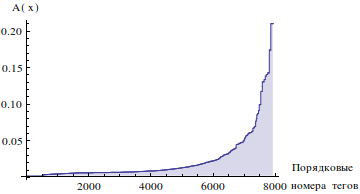
\includegraphics[width=0.5\linewidth]{Dissertation/pics/abstract_words_1}
%    \caption{Значения степени абстрактности}
%  \end{minipage}
%  \label{img:abst_1}
%\end{figure}
%
%\begin{figure}[ht]
%  \begin{minipage}[ht]{1.0\linewidth}\centering
%    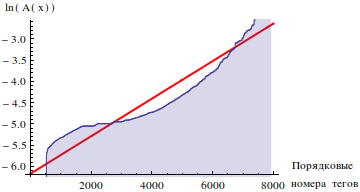
\includegraphics[width=0.5\linewidth]{Dissertation/pics/abstract_words_2}
%    \caption{Значения логарифмов степени абстрактности}
%  \end{minipage}
%  \label{img:abst_2}
%\end{figure}
%

%Формулу, определяющую оптимальное значение степени абстрактности $p$ в окрестность которого попадёт максимальное число искомых тематических ключевых слов, можно представить в следующем виде:

%$$p=\exp{M(\{\log{x}|x = \underset{w}\max{((a_T(w)|w\in t), t \in T})}$$,

%где $T$- коллекция ключевых слов, $a_T(w)$ - абстрактность ключевого слова $w$, $M(x)$ - среднее значение среди $x \in X$

%После определения параметра $p$ остается выбрать интервал, содержащий значение $p$.  Например, можно отступить в обе стороны от $p$ на $\epsilon$ и обозначить множество ключевых слов таких, что $A(x) \in [p − \epsilon,p + \epsilon]$, множеством тематических ключевых слов.

Таким образом, представленный алгоритм позволяет классифицировать каждое ключевое слово системы и определить его как ключевое слово-терми, тематическое ключевое слово или абстрактное ключевое слово. Алгоритм основывается на понятии степени абстрактности ключевого слова, которая была введена ранее. В следующей разделе приводятся результаты тестовых испытаний программной реализации данного алгоритма.

\hl{В следующем подразделе представлено описание алгоритма, определяющего тематику объекта по набору ключевых слов согласно предложенной модели.}

%Значение искомого параметра $p$ в описанном ранее алгоритме оказалось равным $0.0122$.  На чистых данных, для удобства тестирования был выбран интервал $[0.012, 0.013]$. ключевые слова, которые имеют такую степень абстрактности, определены как тематические. Таких ключевых слов обнаружено $65$. В приложении \ref{AppendixB} приводится полный список определенных тематических ключевых слов. Таким образом, алгоритм определил $65$ ключевых слов, из которых $19$ при любых обстоятельствах являются тематическими потому, что это название дисциплин и направлений науки. Еще $13$ ключевых слов субъективно можно считать тематическими. Таким образом точность результата составляет $49.2\%$.

%%\subsection{Определение смысловой близости для решения задачи поиска эксперта} \label{expert_search_wordsim}
%%Постановка и решение задачи поиска эксперта рассматривается далее в главе \ref{expert_search}. Для ее решения появляется необходимость вычислять степень похожести между наборами ключевых слов, характеризующих потенциальных экспертов, с ключевыми словами запроса. Для этого, в свою очередь, разработана базовая процедура для определения близости пары ключевых слов, использующая методы и идеи, которые описаны в настоящей главе.
%%
%%Вычисление смысловой близости пары ключевых слов также основывается на построении графа ключевых слов, введенного в разделе \ref{sect1_1}. Вершины этого графа соответствуют ключевым словам, а взвешенные ребра отражают факт вхождения слов в один набор. Другим важным понятием является уровень абстрактности ключевого слова, который описан в разделе \ref{abstractness}. В этом же разделе представлен алгоритм определения степени абстрактности по ключевому слову Для вычисления смысловой близости пары ключевых слов используются следующие далее соображения.
%%
%%\begin{itemize}
    %%\item \textbf{Чем ближе друг к другу находятся ключевые слова в графе, тем больше они схожи по смыслу.} Другими словами, значение семантической близости обратно пропорционально кратчайшему расстоянию между вершинами в графе. За вес ребра принято число наборов из корпуса, в которые входят оба ключевых слова. Если $w(i, j) = |{p \in W_X | i \in p \wedge j \in W_X}|$ ­ вес ребра ($W_X$ - множество всех наборов ключевых слов информационной системы), то за длину ребра принята величина $l_0(i, j) = \frac{1}{1+\log(w(i,j))}$ , где $i$, $j$ ­ смежные вершины. Для случая $i = j$ положим $l_0(i, i) = 0$. Следует отметить, что от функции $l_0(i, j)$ достаточно потребовать лишь обратной зависимости от функции $w(i, j)$ . Тем не менее, описанная выше формула позволяет получить лучший результат, чем, например, наивная формула $\frac{1}{w(i,j)}$.
    %%\item \textbf{Необходимо использовать только статистически важные связи в графе.} Набор ключевых слов к научной публикации не обязан состоять из похожих по смыслу слов. Например, в одном наборе (<<космический аппарат>>, <<упругие элементы>>, <<процесс отделения>>). Замечается, что ключевые слова <<космический аппарат>> и <<упругие элементы>> не должны обладать сильной семантической связью. Поэтому вводится условие: если количество совместных появлений пары ключевых слов меньше порогового значения $t$ , то такая связь в графе не учитывается. Исключением являются те ребра, удаление которых приводит к увеличению числа компонент связности в графе ключевых слов.
    %%\item \textbf{Пара слов с более высокими степенями абстрактностей должна обладать меньшим значением семантической близости, чем пара узкоспециальных слов.} В качестве примера рассмотрим следующую ситуацию: пара абстрактных по значению ключевых слов («динамика», «кинематика») и пара более узкоспециальных ключевых слов(«прибыль», «доход») могут располагаться на одном расстоянии друг от друга в графе. Однако видно, что пара («прибыль», «доход») явно должна иметь большее значение смысловой близости, потому что оперирует более узкоспециализированными ключевыми словами. Исходя из этих соображений можно предположить, что семантическая близость должна зависеть от уровней абстрактностей сравниваемых ключевых слов.
    %%\item \textbf{Пути графа, проходящие через слова с более высокой степенью абстрактности, должны учитываться с меньшим весом.} Слова, обладающие более широким значением, имеют больше связей с другими словами графа. Это обстоятельство приводит к тому, что существует множество пар узкоспециальных слов, которые явно не являются похожими семантически, однако располагаются при этом близко друг к другу в графе. Обычно такое происходит, если пара слов имеет общую вершину с высокой степенью абстрактности. Например, пара ключевых слов («ленивые вычисления», «оценка максимального правдоподобия») находятся близко друг к другу из­за их связей с ключевым словом «машинное обучение», который является более общим понятием. Можно при этом заметить, что на самом деле слова этой пары далеки друг от друга семантически. По этой причине возникает необходимость «перевзвесить» ребра графа. Обозначим степень абстрактности ключевого слова $x$ за $A(x)$. Величина $A(x)$, исходя из введенного в главе (???) определения, не превышает  1. Положим теперь длину ребра равной $l(i, j) = \exp(\frac{l_0(i, j)}{\log(A(i))\log(A(j))})$. Таким образом, чем выше степени абстрактности вершин, инцидентных данному ребру, тем больше длина этого ребра. Длина кратчайшего пути между вершинами $v_x, v_y$ принята за $L(v_x,v_y)$ . Экспонента в формуле делает значение $l(i, j)$ не меньшим, чем 1.
    %%\item \textbf{Чем больше различных связей (путей) между вершинами в графе, тем больше уровень семантической близости.} При этом дополнительную информацию дают веса ребер. Это следует из того, что если два ключевых слова связаны тяжелым ребром или путь между ребрами имеет большой вес, то такие ключевых слова будут более близки по смыслу, чем аналогичная пара с легкими ребрами. В этой связи возникает необходимость решения задачи определения максимального потока между двумя вершинами графа. В классической постановке требуется для пары вершин, называемых источником и стоком, транспортной сети найти такой поток из источника в сток, что его величина будет максимальна. На граф ключевых слов эта задача переносится очевидным образом, если ребра принять за двунаправленные, а за пропускную способность ребра ­ его вес. При этом пропускная способность считается отдельно для каждого из направлений. Пусть максимальный поток между вершинами $v_x, v_y$ равен $MaxFlow(v_x, v_y)$. Максимальной вместимостью вершины назовем сумму весов ребер, входящих в нее. Обозначим максимальную вместимость вершины $i$ за $C(i)$. Тогда за $F(v_x,v_y)$ примем величину, равную $\frac{MaxFlow(v_x,v_y)}{min(C(v_x), C(v_y))}$. В этом случае $F(v_x,v_y)$ показывает, насколько использована пропускная способность канала между вершинами. Максимум, равный единице, достигается, если пропускная способность использована полностью. В частности, $F(vx,vx) = 1$.
%%\end{itemize}
%%
%%Учитывая перечисленные выше cоображения, формула близости между парой ключевых слов $x$ и $y$ вводится следующим образом:
%%
%%$$ WordSim_{expert}(x, y) = \frac{F(v_x, v_y)}{L(v_x, v_y)}, $$
%%
%%где $v_x$ и $v_y$ - пара вершин в графе ключевых слов, соответствующая ключевым словам $x$ и $y$.
%%


\subsection{Алгоритм выбора тематики объекта} 
В разделе \ref{abstractness} представлена модель классификации ключевых слов на $W$ на три уровня в зависимости от степени абстрактности этих слов. С ее помощью для каждое ключевое слово систему можно отнести к \emph{абстрактным ключевым словам}, \emph{тематическим ключевым словам} или \emph{ключевым словам-терминам}. Множество тематических ключевых слов представляет наибольший интерес, поскольку именно среди них находятся слова, определяющие тематическую направленность объекта. По этой причине  для ключевых слов набора вычисляются степени абстрактности и определяются классы абстрактности, к которым принадлежат слова.

Если в наборе присутствует несколько тематических ключевых слов, то в качестве ответа выдается наиболее абстрактное из них. Следует однако отметить, что во многих наборах тематические ключевые слова отсутствуют. В этом случае для определения тематики объекта используется граф ключевых слов $G_{kw}$, введенный в разделе \ref{sect1_1}. Алгоритм проходит по всем словам набора, начиная с наиболее абстрактного слова и заканчивая словом, обладающим минимальной величиной абстрактности. Для каждого такого слова просматриваются все его соседи в графе ключевых слова $G_{kw}$. Если среди них присутствует хотя бы одно тематическое ключевое слово, то все они возвращается в качестве ответа. В другом случае алгоритм переходит к следующему слову исходного набора.

В том случае, если ни слова исходного набора, ни соседи этих слов в графе $G_{kw}$ не являются тематическими, алгоритм возвращает пустой ответ. Отмечается также, что поиск тематических соседей на расстоянии 2 и более от заданной вершине в графе $G_{kw}$ не приводит к улучшению качества решения задачи. Дело в том, что исходя из соображений из раздела \ref{sect1_1}, семантическая связь между парой вершин очень быстро уменьшается при увеличении расстояния между этими вершинами.

В целях оптимизации вычислений, для множества ключевых слов $w \in W$ коллекции предварительно вычисляются значения степени абстрактности $a(w)$, а также классы абcтрактности $b_w = f_{theme}(a(w))$.

Резюмируя представленные выше соображения, алгоритм выбора тематики представляется в следующем виде.
\begin{enumerate}
    \item Входные параметры алгоритма: набор ключевых слов $t \in T$.
    \item Ключевые слова набора $t$ сортируются по убыванию уровня абстрактности.
    \item Цикл по словам $w$ набора $t$:
        \begin{itemize}
            \item если $b_w = $ \emph{тематическое ключевое слово}, то вернуть его в качестве результата;
            \item иначе, продолжить цикл.
        \end{itemize}
    \item Цикл по словам $w$ набора $t$:
        \begin{itemize}
            \item по графу $G_{kw}$ определяются множество соседей $N_G(w)$ для слова $w$;
            \item если существует такое слово $v$, что $v \in N_G(w)$ и $a_b = $ \emph{тематическое ключевое слово}, то вернуть все такие слова $v$;
            \item иначе, продолжить цикл.
        \end{itemize}
    \item Вернуть пустое множество
\end{enumerate}

Вычислительные затраты на работу программной реализации такого алгоритма оказыва.тся равными $O(nm)$, где $n$ - максимальное число слов в наборе, а $m$ - максимальное число соседей для вершины в графе $G_{kw}$. Первый множитель этой оценки получен в следствии необходимости просмотра всех слов заданного набора. Второй множитель появляется из-за просмотра всех соседей в графе ключевых слов $G_{kw}$.

В следующем разделе \ref{theme_test} демонстрируются результаты работы программной реализации алгоритма на реальных наборах ключевых слов.

%\subsection{Тестовые испытания модели определения абстрактности и тематических ключевых слов} \label{abstr_test}
\subsection{Тестовые испытания} \label{theme_test}

В настоящем подразделе результаты тестовых испытаний программной реализации алгоритмов определения степени абстрактности ключевого слова, тематических ключевых слов  и тематики документа, а также описываются методы предварительной обработки исходных данных и исправления ошибок.  В качестве таких тестовых данных в работе использован корпус ключевых слов научных публикаций. Коллекция представляла собой вручную составленные списки ключевых слов для публикаций технического и гуманитарного профиля, полученные из различных источников, включая сеть Интернет. По этой причине в этих данных присутствовали ошибки и неточности, полученные при их формировании.

По причине того, что данные для тестовых испытаний вводились людьми вручную, было необходимо провести предварительную обработку данных. Предобработка данных - необходимая мера для увеличения точности работы алгоритмов. К мерам, которые применялись для улучшения качества тестовых данных относятся следующие:

\begin{itemize}
    \item все ключевые слова переводились в нижний регистр;
    \item самые популярные из аббревиатур вручную сопоставлялись со своими развёрнутыми формами;
    \item использовалось несколько разделительных символов;
    \item длинные строки без разделителей разделялись по символам пробелов;
    \item в ключевом слове убирался дефис, если уже существует такое же слово без дефиса.
\end{itemize}

При этом замечается, что длинные строки без разделителей в действительности могут представлять собой единственное ключевое слово:

\textbf{[оценка экономического косвенного эффекта от проекта информатизации]}.\

Или же набор ключевых слов, разделенных по пробелу

\textbf{[шахта метан утилизация газогенераторная станция]}.\

По причине того, что длинные ключевые слова встречаются в данных пренебрежимо мало и в соответствующих вершинах построенных графов мало связей, такие длинные одиночные ключевые слова расценивались как множество однословных ключевых слов.

Далее приведен список самых популярных ключевых слов:

\textbf{наночастицы, инновации, метод конечных элементов, механические свойства, динамика, наноструктуры, прочность, научный потенциал, удар, структура, остаточные напряжения, компьютерное моделирование, управление, модель, оптимизация, мониторинг, образование, математическое моделирование, математическая модель, моделирование}

\hl{Популярность некоторых из этих слов является следствием высокой степени абстрактности (к примеру, слово <<моделирование>>). Однако некоторые из них попали в список, потому что некоторая тема может быть популярной (по крайней мере, в рамках рассматриваемой коллекции). По этой причине ключевые слова, относящиеся к этой тематике, могут быть часто использованы в списке ключевых слов (наноструктуры, метод конечных элементов). Однако, по уже представленным ранее данным видно, что наивный алгоритм подсчёта количества вхождений ключевого слова в коллекцию не даёт необходимого результата.}

Далее на Рис. \ref{img:abstr_hist} показано количество наборов, обладающих соответствующей долей неуникальных ключевых слов \hl{(ключевых слов, которые упоминаются хотя бы в двух наборах из коллекции)}. Другими словами, для каждого набора подсчитан процент неуникальных ключевых слов и по этим данным построена гистограмма. Важно отметить, что именно неуникальные ключевые слова дают возможность дальнейшего анализа. Если бы наборы в основном состояли из уникальных ключевых слов, то использование графов и статистического анализа не привело бы к достижению каких-либо значимых результатов. Самое популярное значение доли неуникальных ключевых слов - 2.0. Этот факт означает, что ключевые слова всех наборов этой категории не являются уникальными, несмотря на то, что коллекция состоит по большей части из уникальных ключевых слов. Примером такого набора является:

\textbf{[образование, наука, высшая школа, идеология, математика, филология, история, педагогика, биология]}.

\begin{figure}[ht]
  \begin{minipage}[ht]{1.0\linewidth}\centering
    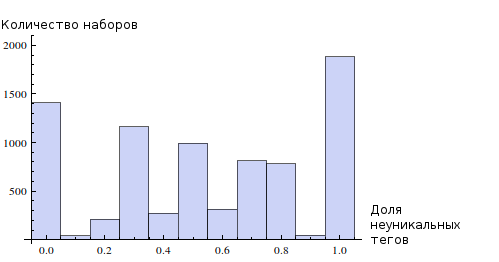
\includegraphics[width=0.5\linewidth]{Dissertation/pics/abstr_hist}
    \caption{Кол-во наборов, с соответсвующей долей неуникальных ключевых слов}
    \label{img:abstr_hist}
  \end{minipage}
\end{figure}

Зачастую ключевые слова наборов такого типа являются очень абстрактными понятиями, что в редких случаях позволяет понять тематику документа. Второе по популярности значение - 0.0. Оно показывает, что существует много наборов, целиком состоящих из уникальных ключевых слов. Причины появления таких наборов состоят в следующем:

\begin{itemize}
    \item ключевые cлова являются слишком узкоспециализированными, например - \textbf{фемтосекундная спектроскопия, лазерные солитоны, дипирролилметаны, подповерхностный радиолокатор};
    \item ключевые слова представлены на другом языке - \textbf{control, sensitivity, equilibria, chaos}.
\end{itemize}

Следует однако отметить, что основная причина именно в узкой специализации ключевых слов.

Между значениями $0.0$ и $1.0$ находится более половины всех наборов. Средняя доля неуникальных ключевых слов по всей коллекции равна $0.53$, то есть, в среднем половина ключевых слов набора встречается в некотором другом объекте коллекции. Типичный набор состоит из нескольких абстрактных ключевых слов, указывающих на общее направление работы и дисциплины, и нескольких ключевых слов, позволяющих понять, о чем конкретно представленный документ.

Исходя из перечисленных выше факторов, представляется возможным изучать методы автоматического определения тематики документа и особенности алгоритмов ассоциативного поиска. При этом логичным инструментарием для решения поставленных задач являются графы, которые были введены в предыдущем разделе. Такие графы будут иметь достаточную связность для дальнейшего анализа и возможности примения алгоритмов, которые представлены в предыдущих разделах.

Для графа ключевых слов, построенного по данным, были определены компоненты связности и вычислены их размеры. Общее число компонент связности - 1856, что, очевидно, очень много для графа из 17428 вершин. Однако, как показывает график на рис.\ref{img:abstr_hist_2} зависимости номера компоненты и её размера (ось ординат логарифмическая), наибольшая компонента связности содержит более половины всех ключевых слов (11558), а вторая по величине имеет лишь 92 вершины. Начиная с 38 позиции, в компонентах содержится менее 10 вершин.

\begin{figure}[ht]
  \begin{minipage}[ht]{1.0\linewidth}\centering
    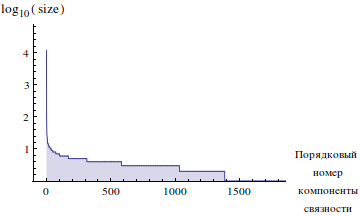
\includegraphics[width=0.5\linewidth]{Dissertation/pics/abstr_hist_2}
    \caption{Распределение размеров компонент связности}
    \label{img:abstr_hist_2}
  \end{minipage}
\end{figure}

\textbf{Дополнительный тестовый набор данных}
По причине того, что имеющийся набор данных недостаточно велик, был разработан алгоритм сбора информации о ключевых словах научных статей из сети Интернет. Для этого был использован API поисковой системы Яндекс, представляющей функциональные возможности получения поисковой выдачи по запросу. Суть алгоритма в следующем.  

На вход алгоритма подается одно ключевое слово <KEYWORD>. В поисковую систему отправляется запрос вида <<mime:pdf keywords: /5 <KEYWORD> >>. Этот запрос означает, что необходимо найти документы формата pdf, в которых после слова «keywords:» на расстоянии не более 5 слов находится заданное слово <KEYWORD>. Поисковая система возвращает сниппеты релевантных документов. Ожидается, что значительная часть сниппетов будет содержать список ключевых слов некоторых научных статей. Производится парсинг сниппетов, выделяются кортежи ключевых слов. Собранные ключевые слова добавляются в множество ключевых слов. Ключевое слово-запрос добавляется в список использованных ключевых слов. Новое ключевое слово <KEYWORD> выбирается из разности множества всех ключевых слов и множества использованных. Действия алгоритма повторяются до тех пор, пока не будет собрана база ключевых слов достаточного размера.

Недостатком программной реализации представленного алгоритма является то обстоятельство, что внешняя поисковая система ограничивает количество запросов в день. По этой причине сбор необходимых данных занимает продолжительное время. Чтобы ускорить процесс, для каждого запроса выкачивается максимально возможное число документов. Как следствие, ключевые слова, по которым строился запрос, встречаются гораздо чаще в собранном множестве ключевых слов. \hl{Такое смещение в данных} негативно влияет на статистические параметры выборки и ухудшает качество работы реализаций алгоритмов. Другой недостаток состоит в том, что если брать слишком большое число документов, то хвост выдачи становится менее релевантен и в выборку добавляются <<мусорные>> данные.

Тем не менее, алгоритм решает важную задачу - восполняет недостаток данных. С помощью программной реализации было собрано более 380000 наборов ключевых слов. Для них были проведены методы предобработки данных, описанные в предыдущем пункте. Кроме того, удалялись наборы без разделителей. Вероятнее всего, такие наборы - это обычные предложения со словом keywords, а также наборы, в которых ключевые слова имеют слишком малую длину (обычно в такие сниппеты попадали инициалы авторов статей). Далее это множество данных обозначается как данные из Веб, а первая коллекция именуется чистыми данными.

\textbf{Результаты тестовых испытаний модели определения абстрактности слова.}

Самые абстрактные слова, полученные при использования программной реализации описанного выше алгоритма на чистых данных, следующие:

\textbf{моделирование, модель, образование, оптимизация, управление, структура, математическая модель, математическое моделирование, мониторинг, прогнозирование, инновации, эффективность, методика, личность, прочность, эксперимент, оценка, история, методы, развитие, анализ, здоровье, инновационная деятельность, культура, качество, свойства, модернизация, синтез, надежность, самоорганизация, адаптация, конкурентоспособность, интеграция, студенты, безопасность, компетенции, взаимодействие, технологии, диагностика, наука, государство, компьютерное моделирование, инновационное развитие, устойчивость, компетентностный подход, динамика, технология, высшая школа, нано-
частицы, метод конечных элементов.}

В целом получены неплохие по оценке квалифицированных экспертов результаты. Из выделенных слов значительную часть можно назвать абстрактными в некотором смысле. Смешивание помогло избавиться от явных выбросов в каждом из алгоритмов и несколько усреднить результат. Тем не менее, добиться заметного повышения качества за счет таких действий не удалось, поскольку представленные алгоритмы имеют одну природу и решают схожие задачи. По этой причине они зачастую ошибаются на некоторых данных одновременно, что влечет за собой ошибку в результатах работы общего алгоритма.

\hl{Результаты работы программной реализации алгоритма на дополнительном наборе данных из Веб, описание которого приведено ранее, следующие:}

\textbf{development, data mining, environment, evaluation, model, management, machine learning, modelling, growth, reliability, neural networks, design, stability, learning, security, uncertainty, clustering, education, performance, modeling, optimization, simulation.}

Для этого набора получены схожие по качеству результату. Однако можно заметить, что некоторые слова определяются абстрактными по причине того, что они были использованы в поисковый запросах, с помощью которых был собран дополнительный тестовый набор данных. Таким словом, например, является термин «machine learning» , который не должен был войти в множество абстрактных слов.

\textbf{Результаты тестовых испытаний модели определения тематических ключевых слов.}
Для тестирования было выбрано $65$ ключевых слов на чистых данных. Ключевые слова, которые имеют степень абстрактности в отрезке $[0.012, 0.013]$, определены как тематические. В приложении \ref{AppendixB} приводится полный список определенных тематических ключевых слов. Таким образом, алгоритм определил $65$ ключевых слов, из которых $19$ при любых обстоятельствах являются тематическими потому, что это название дисциплин и направлений науки. Еще $13$ ключевых слов субъективно можно считать тематическими. Таким образом точность результата составляет $49.2\%$.

\hl{Такой уровень точности можно считать удовлетворительным, принимая во внимание тот факт, что разработанная модель не использует никаких априорных знаний о тематике ключевых слов. Другими словами, в ходе построения модели не были использованы внешние источники данных, такие как тезаурусы, содержащие в себе информацию о степенях абстрактности слов и их тематической направленности. Это обстоятельство позволяет утверждать об универсальности исследуемого подхода с точки зрения применимости к произвольным наборам данных. Становится возможным определение тематических ключевых слов для коллекций различной природы (наукометрия, данные социальных сетей и пр.), предметной направленности (технические, гуманитарные науки) и степени специализированности (узкопрофильные системы и системы общего назначения).}


\textbf{Результаты тестовых испытаний модели определения тематики документа.}
Тестирование программное реализации алгоритма проводилось на данных, описанных ранее. Некоторые из результатов приведены в таблице \ref{tbl:theme_table}.

\begin{table}[H]
\small
\begin{tabularx}{16cm}{|X|X|} 
        \hline
        Набор ключевых слов & Возможная тематика набора \\ \hline 
        выпуклое программирование, принцип лагранжа, теорема куна-таккера в недифференциальной форме, параметрическая задача, минимизирующая последовательность, двойственность, регуляризация & оптимальное управление \\ \hline
        состояние метакультуры, культуры среды, границы, этика творчества, личность & биометрия, массовая культура, педагогическая деятельность \\ \hline 
        окружающая среда, биосферная совместимость, система жизнеобеспечения & гидродинамика, факторный анализ \\ \hline
        персонализированное обучение, подготовка учителя информатики, синергетический подход & конструирование, педагогическая деятельность \\ \hline
        жидкие кристаллы, ориентирующие слои, аморфный гидрогенизированный улерод & жидкие кристаллы \\ \hline
        прогноз, формы предвидения, интерпретация темпоральных модусов, аксиология, социальное противоречие & конструирование, массовая культура \\ \hline
        металлические материалы, термическая обработка, структура, свойства & конструирование, физическое моделирование \\ \hline
        инклюзия, инвалидность, сопровождение, студенты-инвалиды  & массовая культура \\ \hline
        модуль выпуклости, равномерно выпуклая функция, равномерно выпуклое множество & [не определено] \\ \hline
        урбанизированная территория, гуманитарный баланс, корреляция регрессия математическая модель & биометрия, кинематика, конструирование, нелинейные колебания, физическое моделирование \\ \hline
        \caption{Наборы и предсказанные им тематические направления} \label{tbl:theme_table}
\end{tabularx}
\end{table}

%\begin{figure}[ht]
  %\begin{minipage}[ht]{1.0\linewidth}\centering
    %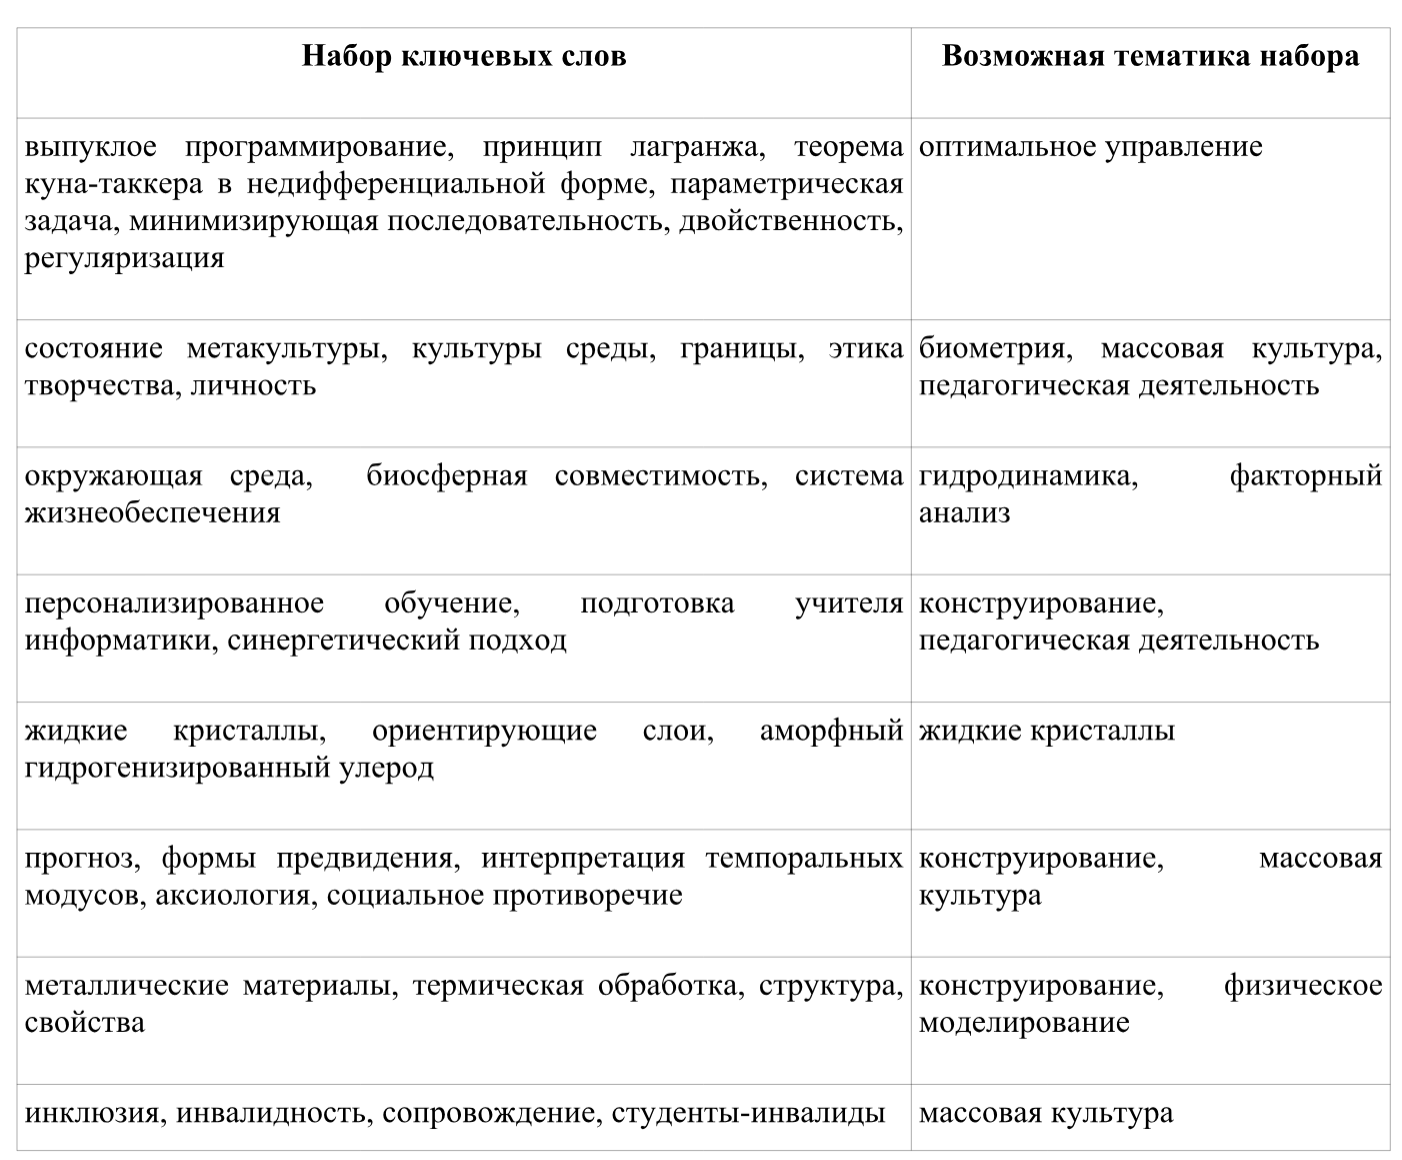
\includegraphics[width=1.0\linewidth]{Dissertation/pics/theme_table_1}
  %\end{minipage}
  %\label{tbl:theme_table_1}
%\end{figure}

%\begin{figure}[ht]
  %\begin{minipage}[ht]{1.0\linewidth}\centering
    %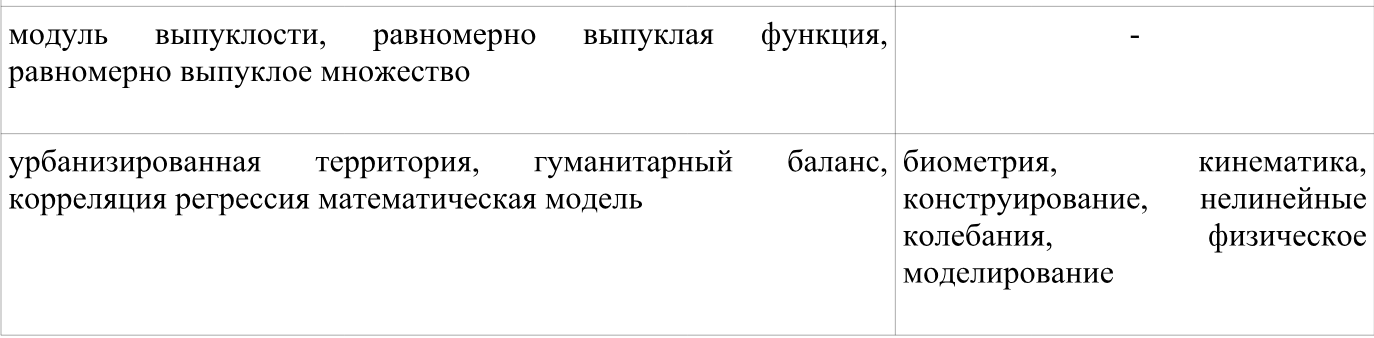
\includegraphics[width=1.0\linewidth]{Dissertation/pics/theme_table_2}
    %\caption{Наборы и предсказанные им тематические направления}
  %\end{minipage}
  %\label{tbl:theme_table_2}
%\end{figure}

В первом примере показано верное определение тематики. При этом можно заметить отсутствие тематического ключевого слова в исходном наборе. Последние два примера демонстрируют случаи, когда тематическое ключевое слово не определено или определено слишком большое число таких слов.

\hl{Отмечается также, что рассмотренные примеры подбирались из условия, что в самом наборе отсутствуют тематические ключевые слова. Такая мера делает тестовое испытание более содержательным, поскольку в этом случае требуется найти наиболее подходящие тематические ключевые слова во всей рассматриваемой коллекции слов. По экспертным оценкам получен адекватный уровень качества работы программной реализации алгоритмов.}

\hl{В следующем далее подразделе сформулированы основные выводы и предложены идеи для дальнейшего развития данного подхода.}

\subsection{\hl{Выводы}}

\hl{В данном представлено описание моделей, алгоритмов, а также реализующих их программных комплексов, решающих задачу определения тематической направленности объекта информационно-аналитической системы.}

В целом, следует отметить, что алгоритм достаточно часто ошибается. Во многих случаях ошибки возникают на наборах, состоящих только из редких слов-терминов. Причина в том, что слова в подобных наборах не соединены напрямую с тематическими, а увеличение пути сильно уменьшает качество результатов. Не определяется тематика и у тех наборов, ключевые слова которых попали в малые компоненты связности без тематических ключевы слов. Однако основная трудность - это накопление ошибок разных алгоритмов. Сначала слово ошибочно получило высокий уровень абстрактности, затем попал в список тематических и, в итоге, неправильно определена тематика набора.

Несмотря на отмеченные недостатки, предложенный подход потенциально может быть улучшен. Для этого можно использовать все ключевые слова из набора для определения тематики, проверять абстрактности вершин на пути от данного ключевого слова к тематическому и использовать многие другие эвристики. Однако уже сейчас можно констатировать, что алгоритм способен с некоторой адекватной точностью решать поставленную задачу. 


\section{Решение задачи поиска экспертов} \label{expert_search}

В данном разделе представлено описание моделей, алгоритмов и программных комплексов, решающих востребованную практикой задачу поиска эксперта. В рамках этой задачи необходимо по запросу, состоящему из набора ключевых слов, находить наиболее релевантные объекты информационно-аналитической системы, наилучшим образом удовлетворяющие исходному запросу. Задача поиска эксперта является важной для наукометрических систем, поскольку позволяют существенно улучшить качество поиска необходимой пользователю информации. Модели и их программные реализации, описанные в настоящем разделе, прошли опробацию в системе ИАС <<Истина>>.

\subsection{Постановка задачи}
Рассмотрим математически формализованную постановку задачи. Дано множество экспертов системы $E$ и множество ключевых слов $W$. Каждый эксперт $e_i \in E$ представлен набором ключевых слов $t_i \in T$, состоящим из $k_i$ ключевых слов из множества $W$. наборов ключевых слов $W_X$ и объектов информационной системы $X$, а также множество $Q$ запросов к системе. Обозначим за $W$ множество всех уникальных ключевых слов из всех наборов $W_X$. Каждый элемент $x_i \in X$ множества объектов ассоциирован с набором ключевых слов $W_i = \{w_{i_0}, w_{i_1}, ..., w_{i_{n_i}} \} \in W_X \in 2^W$. Точно также каждый запрос $q_j \in Q$ связан с некоторым набором ключевых слов $W_j = \{w_{j_0}, w_{j_1}, ..., w_{j_{n_j}} \} \in 2^W$. Необходимо определить меру близости пары запрос­объект для каждого объекта и каждого запроса, т.е.  функцию $f : Q \times X \rightarrow R$. Поскольку запросам и объектам единственным образом сопоставляются наборы ключевых слов, то задача сводится к определению меры близости на наборах: $f_w : 2^W \times 2^W \rightarrow R$. Кроме того, необходимо разработать эффективный алгоритм, который, используя меру близости и некоторые дополнительные идеи, мог бы по запросу выдавать множество объектов, наиболее релевантных данному запросу.
\subsection{Процедура поиска экспертов}
По данному множеству наборов ключевых слов (множеству экспертов) строится граф ключевых слов. Далее необходимо для каждого ключевого слова $x$ найти ближайшие по смыслу слова. Мера близости слов вычисляется сначала между тегом $x$ и его соседями в графе, после чего просматриваются соседи соседей $x$ и так до тех пор, пока не наберется фиксированное число кандидат. Часть наиболее релевантных тегов сохраняются, как наиболее близкие к $x$. В дополнение к этому, строится инвертированный индекс, который позволяет по слову восстановить наборы, содержащие это слово. После того, как в систему приходит запрос, для каждого слова из запроса выгружаются ближайшие по смыслу слова и первоначальный запрос расширяется. Затем по словам из расширенного запроса восстанавливаются наборы­кандидаты. Для каждого из них считается мера близости с исходным запросом $TupleSim_{expert}$, подробно описанная в \ref{expert_search_tuplesim}. В конце своей работы алгоритм возвращает наиболее релевантные наборы­кандидаты.

\section{Построение тезауруса ключевых слов по коллекции наборов} \label{thes}

% >>> SYNOPSIS_2.4
В данном разделе описывается построение тезауруса ключевых слов по коллекции наборов ключевых слов. Схема построения построения приводится на рисунке \ref{img:thes}.

\begin{figure}[ht]
  \begin{minipage}[ht]{1.0\linewidth}\centering
    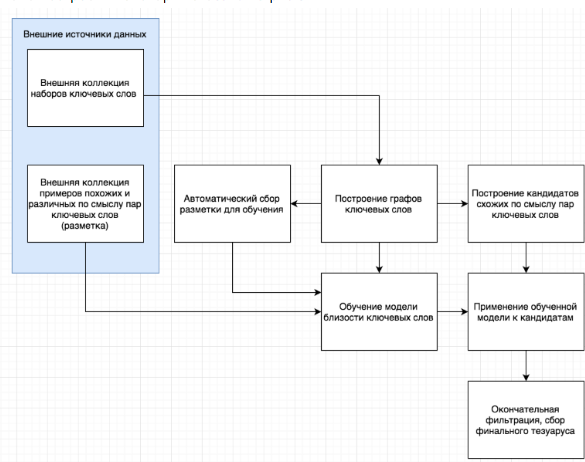
\includegraphics[width=0.7\linewidth]{Dissertation/pics/thes}
    \caption{Схема построения словаря тезауруса ключевых слов}
    \label{img:thes}
  \end{minipage}
\end{figure}

В качестве внешних данных используется коллекция наборов ключевых слов научных публикаций, собранная из сети Веб. Это коллекция, насчитывающая сотни тысяч наборов ключевых слов для русскоязычных статей и миллиона наборов на английском языке. С помощью этих наборов поочередно строится несколько графов близости. Одним из таких графов является, например, граф, в вершинах которого находятся ключевые слова, а в ребро означает причастность двух ключевых слов одному набору. Вес ребра тем больше, чем чаще пара слов встречается в одном наборе. Другим примером контекстного семантического графа является граф, в вершинах которого как и прежде стоят ключевые слова, а ребра указывают на наличие у этой пары общего ключевого слова, которое входит в некоторые наборы вместе и с первым словом из пары, и со вторым (но не с двумя сразу). Было показано, что ребра такого графа гораздо сильнее отражают семантическую близость, в то время как ребра первого графа служат для улучшения механизмов поисковых подсказок, потому что предлагают связанные, но более разнообразные слова для заданного.

% SYNOPSIS_2.4 <<<

Также внешними данными является коллекция достоверно похожих и различных пар ключевых слов (разметка). Такая разметка необходима для настройки алгоритмов и тестирования качества их программных реализаций. В эту разметку входят открытые базы синонимов, антонимов, аббревиатур, а также некоторые переводы на другие языки.

Помимо словарной разметки, при построении тезауруса на базе графов ключевых слов генерируется автоматическая разметка. Преимущество этой разметки в том, что она полностью строится по данным, что означает отсуствие необходимости иметь внешнюю собранную вручную разметку (обычно это дорогой и трудоемкий процесс). Вместе с этим, автоматическая разметка не вносит смещение в данные. Например, если в базах синонимов встречается много математических терминов, но мало биологических, то модель настроится на то, чтобы давать парам математических терминов большее значение близости. 

В то же время автоматическая разметка будет использовать обучающие примеры из разных областей ровно в той пропорции, в которой они представлены в конкретных данных. С другой стороны, такая разметка может быть менее точной, поэтому в финальной версии алгоритма используется обе разметки.

Поскольку ключевых слов достаточно много, то рассмотреть все пары не представляется возможным. Как следствие, по построенным графам строятся кандидаты близких по смыслу пар ключевых слов. Их количество достаточно велико, но значительно меньше всех возможных пар.

После этого для пар-кандидатов подсчитываются числовые факторы: различные расстояния и характеристики в графе, статистические показатели и другие. По этим факторам строится модель, которая настраивается с помощью разметок, описанных выше. Затем модель применяется к парам-кандидатам и те пары, которым модель дала наибольший вес, проходят в окончательный словарь ключевых слов.


\section{Реализация поиска по ключевым словам на базе собранного тезауруса синонимов}
Программные механизмы использования ключевых слов позволяют существенно улучшить поиск необходимой пользователю информации в системе. Информацию о большинстве объектов системы (публикации, конференции, сведения о пользователях и др.) можно дополнить произвольным набором ключевых на естественном языке. После внесения информации, происходит индексирование и обработка ключевых слов, что позволяет проводить дальнейший интеллектуальный анализ данных с целью получения релевантного ответа на запрос.

Основные задачи, которые могут быть решены при помощи ключевых слов - улучшение качества поисковых алгоритмов ранжирования подлежащих анализу объектов, а также поисковые подсказки рекомендательного характера для пользователя.

Для решения обозначенных выше задач был реализован поисковый модуль на базе фреймворка Django. Он представляет собой поисковую строку, в которую вводятся ключевые слова, разделенные запятой, а также таблицы поисковой выдачи, в которой указаны объекты, удовлетворяющие критериям поиска, в порядке убывания релевантности. В момент ввода пользователю предлагается расширить свой запрос некоторыми связанными ключевыми словами, что впоследствии помогает найти более релевантные запросу объекты. Интерфейс системы представлен на рис.\ref{img:search}

\begin{figure}[ht]
  \begin{minipage}[ht]{1.0\linewidth}\centering
    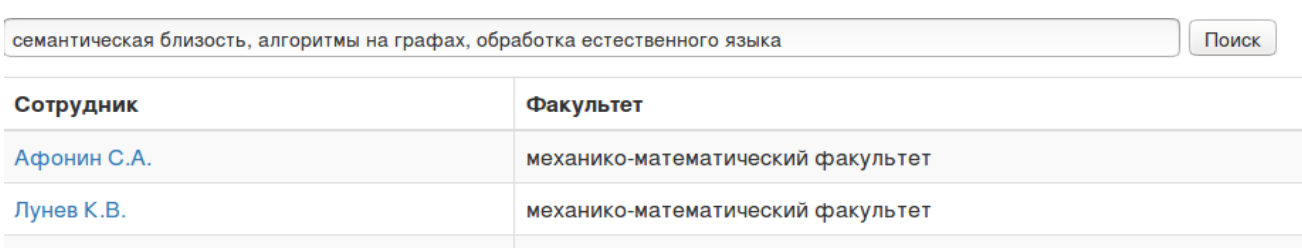
\includegraphics[width=0.95\linewidth]{Dissertation/pics/search}
    \caption{Интерфейс модуля поиска по ключевым словам}
  \end{minipage}
  \label{img:search}
\end{figure}

Помимо этого реализовано ядро подсистемы обработки ключевых слов, которое проводит основной анализ, определение семантической близости пары слов, подготовку тезауруса ключевых слов. Методы определения сематнической близости пары ключевых слов описаны в главе \ref{chapt_word_similarity}, а описание алгоритма построения тезауруса дано в разделе \ref{thes}. Код ядра представляет собой модули, процедуры и скрипты на языке Python с использованием открытых математических пакетов (Numpy, Pandas, Scipy), а также пакетов для анализа данных и машинного обучения (Scikit-learn, XGBoost). Данный модуль может использоваться отдельно от основного кода системы.

\begin{figure}[ht]
  \begin{minipage}[ht]{1.0\linewidth}\centering
    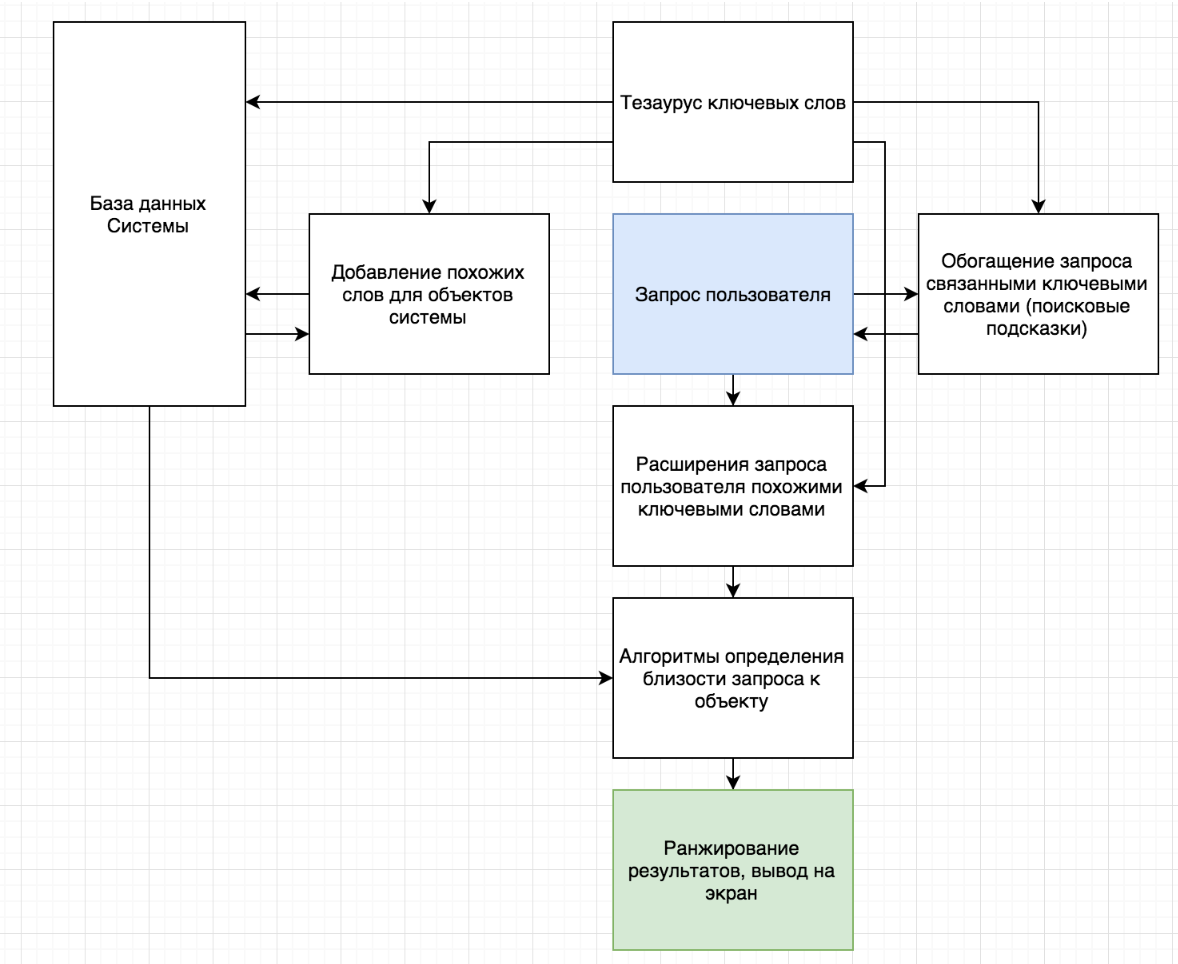
\includegraphics[width=0.95\linewidth]{Dissertation/pics/search_2}
    \caption{Схема обработки запроса на поиск по ключевым словам}
  \end{minipage}
  \label{img:search_2}
\end{figure}

На рис.\ref{img:search_2} представлена схема выполнения и обработки запроса. Основной процесс работы с ключевыми словами состоит из трех шагов. На первом из них в ядре модели рассчитывается тезаурус ключевых слов. В этом тезаурусе для каждого ключевого слова хранятся ключевые слова, близкие по смыслу к данному, с указанием значения меры близости. Далее полученный словарь загружаются в базу данных системы, после чего появляется возможность по введенному пользователем слову быстро восстанавливать множество ключевых слов, похожих на заданное. Данный этап сбора словаря стоит обособленно от процесса поиска и может быть перезапущен в любой момент времени. 

Второй шаг - обогащение объектов системы ключевыми словами из собранного на прошлом шаге тезауруса. Если для объекта указан набор ключевых слов, то для к каждому из этих ключевых слов добавляется информация о близких словах из тезауруса. Данный этап также является шагом предобработки данных. 

Последний этап - непосредственно поиск по ключевым словам. Введенный пользователем запрос расширяется словами тезауруса, далее происходит поиск сущностей по расширенным наборам ключевых слов (как в запросе, так и в описании объекта). Для найденных объектов вычисляется релевантность (функция, возвращающая действительное число по паре запрос-объект, большие значения которой соответствуют более релевантным объектам), результаты сортируются по убыванию релевантности и выводятся на экран пользователя. Использование поискового запроса пользователя как набора ключевых слов, позволяет применять упомянутые выше алгоритмы для разработки поисковых подсказок. Такие подсказки предлагают пользователю дополнить свой запрос ключевыми словами, связанными по смыслу с теми, которые он уже ввел.

Трудностью в решении задачи реализации поиска по ключевым словам является тот факт, что для значительной части слов в системе нет достаточной статистики их использования. Как следствие, возникает ситуация, когда про слово, добавленное к описанию объекта или про слово, заданное пользователем в поисковую строку, нет достаточной информации, что не позволяет получить релевантную запросу поисковую выдачу. Для преодоления этой трудности в системе реализованы интеллектуальные алгоритмы анализа ключевых слов, а также используются внешние корпусы данных на естественном языке, описанные в разделе \ref{ml_sim}. Основными направлениями работы по использованию ключевых слов для выполнения поисковых запросов являются следующие:

\begin{itemize}
    \item определение семантической близости между парой ключевых слов с помощью алгоритмов машинного обучения и внешних наборов данных;
    \item определение семантической между парами наборов ключевых слов;
    \item использование связей между объектами системы (например, списки публикаций одного автора, таблицы соавторства, списки участников конференции, работников лаборатории и др.)
\end{itemize}

Таким образом, поиск по ключевым словам осуществляет не только определение точного вхождения слов запроса в слова объектов, по которым ведется поиск, но также происходит расширение как запроса, так и подлежащих анализу документов семантически близкими словами. В дополнении к этому, наборы ключевых слов, ассоциированные с объектами системы, обогащаются словами, от связанных с ними объектов. Все это позволяет увеличить описание к имеющимся данным и, следовательно, улучшить возможности поиска. 


%\subsection{Поисковые подсказки для ключевых слов}
%Поисковые подсказки позволяют облегчить пользователю формулировку запроса к системе на естественном языке. Стандартные алгоритмы построения поисковых подсказок позволяют выбрать необходимое слово по его введенному префиксу. Но во многих ситуациях является важным подсказать пользователю слово, близкое по значению к вводимому. Такое слово пользователь, возможно, не вспомнил во время ввода запроса. Алгоритм полезен также и в тех случаях, когда пользователь планировал ввести предлагаемое слово, поскольку это экономит время ввода: нет необходимости полностью вводить слово, его можно просто выбрать из списка предложенных слов.

%Поэтому была реализована система поисковых подсказок, описание которой приведено далее:
%\begin{itemize}
    %\item известные системе ключевые слова кладутся в префиксное дерево;
    %\item в листья префиксного дерева кладутся ссылки на ключевые слова, близкие к слову, построенному от вершины дерева до этого листа;
    %\item при вводе пользователем слова, в интерфейсе появляется список возможных завершений данного слова, построенный обходом от текущей вершины в префиксном дереве;
    %\item при достижении листовой вершины (путем полного ввода слова или выбора подсказки) в интерфейсе показывается список слов, близких по смыслу к только что введенному. Слова этого списка отсортированы по уменьшению значения функции семантической близости;
    %\item при выборе одного из слов из списка семантически близких к введенному, это слово добавляется в запрос. Пользователю предлагается выбрать близкие слова к только что добавленному или начать вводить следующее слово самостоятельно.
    %\item при нажатии на кнопку <<Поиск>> начинается процесс построения поисковой выдачи по введенному запросу.
%\end{itemize}

\section{Соответствие программного модуля интеллектуального анализа на основе ключевых слов предъявляемым требованиям}
В настоящем разделе показаны результаты анализа разработанного автором программного модуля на соответствие требованиям, заявляенным в приложении \ref{AppendixRequirements}. Здесь и далее верхнеуровневыми моделями называются модели, решающий практические задачи, описание которых предложено в данной главе. Нижнеуровневыми являются те модели, описанные в главах \ref{chapt_word_similarity}, \ref{chapt_tuple_similarity}. Далее приводятся формулировки требований и комментарии о степени их выполнения.

\begin{enumerate}
    \item \textbf{Функциональные требования.}
    \begin{enumerate}[label*=\arabic*.]
        \item \textbf{Наличие для каждого из используемых в модуле интеллектуального анализа на основе ключевых слов программного средства строго описанных алгоритмов, на которых они реализованы и моделей, в рамках которых эти алгоритмы построены.}

            Описание всех необходимых моделей было приведено в данной и предыдущих главах настоящей диссертации. Для разработанных программных реализаций проведены тестовые испытания, для основных алгоритмов получены оценки производительности и потребления памяти. Таким образом данное требование является выполненным.
        \item \textbf{Эффективное обновление имеющихся и добавление новых данных в систему.}

            Наиболее сложным для обновления является процесс добавления новых ключевых слов в систему. Под <<новыми>> в данном случае понимаются те слова, которые не встречались ранее ни в одном из наборов ключевых слов. Причиной этому является тот факт, что ключевые слова - базовые единицы всех разработанных моделей, поэтому при добавлении новых ключевых слов в систему необходимо пересчитать все верхнеуровневые модели. В программном комплексе имеется две способа обновления данных. Первый из них заключается в пересборке всего набора моделей с самого начала. Такой способ применим для систем небольшого размера (до 25000 объектов). Второй способ - проведение частичного обновления по уже построенной системе. В этом случае новые ключевые слова добавляются в существующие графы, после чего для этих слов вычисляются необходимые меры семантической близости. Отмечается, что такой подход менее эффективен с точки зрения временных затрат на одно ключевое слово, поскольку использует более наивные методы вычисления. Однако, в случае больших по объему имеющихся данных систем этот способ позволяет быстрее провести обновление системы. 

            Добавление новых наборов ключевых слов не требует дополнительной ресурсозатратной по объему операций предобработки, если в новых наборах нет новых ключевых слов. Добавление новых отношений в систему также является эффективной операцией.
            
            Следует также отметить, что перерасчет всех моделей даже для больших систем занимает не более суток. Время выполнения подготовительных процедур составляет 7 часов на входном объеме данных в 300000 наборов. Таким образом, при ежедневном пересборе моделей, изменения в семантических моделях дойдут до пользователей системы на следующий день. Для сложных интеллектуальных моделей и систем, содержащих сотни тысячи и миллионы сущностей, данный период обновления можно считать допустимым. Исходя из вышеизложенного, требование является выполненным.

        \item \textbf{Эффективная процедура кластеризации ключевых слов системы и поиск необходимого кластера.}

            Процесс кластеризации занимает не более получаса даже на больших наборах данных (миллионы наборов ключевых слов). Следует отметить, что необходимость в перекластеризации данных не возникает слишком часто, поэтому время работы алгоритма является удовлетворительным. Поиск необходимого кластера эффективен засчет хранения ключевых слов в системе. Таким образом, требование является выполненным.
        \item \textbf{Эффективный поиск похожих объектов с помощью обученных моделей.}

            Вся необходимая семантическая информация подсчитывается на этапах предобработки, что позволяет сделать этап поиска быстрым. Данное требование является выполненным.

        \item \textbf{Реализация подмодулей, решающих практически значимые задачи информационного поиска в рамках аналитической системы.}

            Описание необходимых модулей представлено в данной главе, поэтому требование является выполненным.

        \item \textbf{Сбор пользовательской информации в ходе взаимодействия с комплексом.}

            Для решения задачи используется готовый подмодуль логирования фреймворка Django. Отмечается при этом, что разрабатываемые модули не реализуют базу данных для системы, в которую они внедряются. Другими словами, эффективное хранение ключевых слов и наборов ключевых слов должно быть реализовано на стороне интеллектуальной системы, а разрабатываемые автором модули хранят в себе вычисленную семантическую информацию, вспомогательные данные, собранные тезаурусы и специфическ представления для взаимосвязанных объектов. 
            
            Кроме того, для последующего улучшения качества разработанных моделей проводится сбор данных о пользовательских действий. Такие действия дают важную обратную связь от пользователя, помогают понять насколько правильным было решение показать пользователю ту или иную информацию. Примером таких действий может быть факт клика пользователем на конкретный результат поиска по его запросу. Если пользователи часто выбирают первую строчку в результатах поиска, то это означает, что программный модуль нашел необходимые объекты по данному запросу. Исходы из вышесказанного, требование считается выполненным.

        %\item \textbf{Соответствие принятым в индустрии соглашениям и стандартам.}

            %Основная часть программного кода реализована на языке Python 

        \item \textbf{Система должна функционировать под управлением ОС с открытым исходным кодом.}

            Разработанный программный модуль функционирует под управлением ОС семейства Linux, поэтому требование считается выполненным.
    \end{enumerate}

    \item \textbf{Надежность.}
    \begin{enumerate}[label*=\arabic*.]
        \item  \textbf{Качество обученных моделей должно валидироваться на отложенных выборках после каждого изменения моделей.}

            Для моделей вычисления семантической близости ключевых слов были разработаны обучающие выборки, описание которых приводится в \ref{art_train}. Кроме того, для моделей выполняется ряд тестовых испытаний, описанных в соответствующих разделах главы \ref{chapt_word_similarity}. Тестирование при этом не применяется к тем данным, на которых обучались модели, другими словами, для валидации используется отложенная выборка данных. 
            
            Валидация остальных моделей проводится по зафиксированным примерам и правильным ответам для них, которые набирались группой экспертов.

            Процесс обучения прекращается, если хотя бы в одном из тестов качество модели упало хотя бы на 10\%. 

        \item  \textbf{Стабильная работа в условиях одновременного использования сотрудниками крупной организации.}

             Использование разработанных высокоуровневых семантических моделей не требует больших вычислительных мощностей, поскольку все необходимые данные, а также модели нижнего уровня являются подготовленными. Это обстоятельство позволяет получать нужные результаты применения программных реализаций одновременно большому количеству сотрудников. Следовательно, данное требование выполнено.

        \item  \textbf{Устойчивость к программным ошибкам и ошибкам интерфейса.}

            Программные реализации моделей устроены таким образом, чтобы при возникновении ошибок программа выдает некоторые значения по умолчанию. Факт ошибки при этом логируется программным модулем. Такого же поведения придерживается модуль, если нужная модель не выдает ответ слишком долгое время. Таким образом, реализованное поведение по умолчанию выполняет требование.
    \end{enumerate}

    \item \textbf{Практичность.}
    \begin{enumerate}[label*=\arabic*.]
        \item \textbf{Комплекс должeн иметь простой интуитивный интерфейс для пользователя.}

            На данном этапе разработки модуля пользователь обладает минимальным интерфейсов для задания запроса. Данное требование выполнено.

        \item \textbf{Комплекс должeн быть легко читаемым и понимаемым для разработчиков.}

            Комплекс разработан на языке Python, читаемость кода которого была заложена разработчиками языка. Код разработан в объектно-ориентированном стиле, что позваляет инкапсулировать внутренние методы и переменные. Для математических вычислений используются удобные библиотеки с открытым исходным кодом и обширной документацией. Код реализован согласно стандарту \emph{PEP8}. Данные стандарт дает рекомендации по написанию грамотного и легкочитаемого кода. Основные неоднозначные моменты в коде имеют поясняющий их комментарий. В этой связи, требование является выполненным.

        \item \textbf{Комплекс должен включать средства обратной связи пользователя с разработчиками.}
            Все пользовательские действия логируются разработанным модулем, задача явной обратной связи пользователя с разработчиком решается основной интеллектуальной системой, в которую внедряется реализованный модуль. Таким образом, требование выполнено частично.

    \end{enumerate}
    \item\textbf{Эффективность.}
    \begin{enumerate}[label*=\arabic*.]
        \item \textbf{Удовлетворительные показатели качества работы моделей на сильно ограниченных по объему данных.}

            Эффективность работы моделей на небольших объемах данных продемонстрирована в подразделах <<Тестовые испытания>> соответствующих разделов. Получены удовлетворительные показатели качества, поэтому требование считается выполненным.

        \item \textbf{Этап предподготовки комплекса.}

            Этапы предподготовки данных, обучения и настройки моделей, а также  подготовки ресурсов, используемых непосредственно верхнеуровневыми моделями на объемах данных, для систем, включающих в себя сотни тысяч сущностей, занимает порядка 10 часов на ЭВМ, обладающей 24-ядерным процессором и 64Гб оперативной памяти. Таким образом, и добавление новых сущностей, и перевычисление всех элементов комплекса укладывается в период в несколько часов, что выполняет предъявляемое требование.

        \item \textbf{Этап использования моделей.}

            В то время, как выдача нужного кластера ключевых слов и вычисление поисковых подсказок занимают доли секунды, построение полной поисковой выдачи имеет точки для роста производительности. Тем не менее, благодаря предрасчету данных и моделей, поисковые вычисления происходят с удовлетворительной скоростью. Поэтому требование считается выполненным частично.

    \end{enumerate}
    \item \textbf{Сопровождаемость.}
    \begin{enumerate}[label*=\arabic*.]
        \item  \textbf{Весь комплекс архитектурно должен разбиваться на ряд отдельных модулей. Логика и параметры этих модулей системы должны быть инкапсулированы друг от друга.}

            Код разработан в объектно-ориентированном стиле, что позваляет инкапсулировать внутренние методы и переменные. Реализована иерархическая структура использования моделей: верхнеуровневые классы, решающие заявленные практические задачи, используют модели семантической близости объектов системы, которые, в свою очередь, используют модели семантической близости пары наборов ключевых слов. На самом низком уровне модели для пар наборов ключевых слов используют модели семантической близости пары ключевых слов. При этом прямого доступа из моделей верхнего уровня к моделям нижнего уровня разработчикам не дается. Это упрощает понимание кода и делает разработку более эффективной. Обозначенные выше доводы позволяют считать требование выполненным.

        \item  \textbf{Иметь возможность быстрого и эффективного способа расширения функционала комплекса.}
            
            Ввиду обособленности реализаций различных моделей, а также объектной ориентированности кода, расширение имеющогося функционала не должно вызывать проблем у разработчиков. По этой причине требование считается выполненным.

        \item  \textbf{Быть документированной.}

            Основные классы и функции задокументированны. Кроме того, описан формат входных и выходных данных для каждой модели. Тем не менее, не все места в программном коде имеют исчерпывающую документацию, поэтому требование принимается выполненным частично.

    \end{enumerate}
    \item \textbf{Мобильность.}
    \begin{enumerate}[label*=\arabic*.]
        \item \textbf{Возможность внедрения в различные информационно-аналитические системы произвольной направленности с допустимым уровнем качества моделей. Модели должны иметь возможность обучаться на данных новой системы.}

            Единственным необходимым требованием к системе является наличие ассоциированных ключевых слов к сущностям этой системы. В дополнении к этому, обогащение моделей с помощью информации о взаимосвязанных объектах может дать значительный рост эффективности верхнеуровневых моделей.
        
        \item \textbf{Возможность обучения специфических моделей семантической близости, автоматически подстраиваемых к предметной области системы, в которой разворачивается комплекс.}

            Модели разрабатывались из условий максимальной независимости от внешних данных. Семантическая информация, которую определяют эти модели, целиком берется из тех данных, в которых они обучаются, поэтому требование подстраиваемости под конкретную область выполнено.

        \item \textbf{Возможность обучения моделей семантической близости без имеющихся обучающих примеров.}

            Модели вычисления семантической близости для пары ключевых слов, а также модель кластеризации ключевых слов способны обучаться в полностью автоматическом режиме, другим же необходимы обучающие примеры, заданные экспертной группой, поэтому данное требование удовлетворено частично.

        \item \textbf{Возможность внедрения в систему с дефицитом данных о ключевых словах.}

            Дефицит информации приводит к деградации качества разработанных моделей. Отмечается при этом, что разработанные решения демонстрируют адекватные результаты на небольших объемах данных, начиная от 1000 наборов ключевых слов. Дополнительным источником качества в случае дефицита данных служит информация о взаимосвязанных объектах. Поскольку возможность внедрения присутствует, требование считается выполненным.

        \item \textbf{Адаптируемость к добавлению новых сущностей и отношений между ними в системе.}

            Благодаря возможности дообучения, а также возможности относительно быстро пересчитать все требуемые модели с начала, данное требование считается выполненным.

        \item \textbf{Развертываемость комплекса внутри новой системы не должна занимать много времени работы экспертов. Необходимо лишь наладить поставку данных в нужном формате и сконфигурать модули для наиболее эффективного решения задач конкретной системы.}

            На текущей момент высокоуровневые модели требуют небольшое количество экспертной информации из предметной области для правильной настройки моделей. Поэтому требование считается выполненным частично.

        \item \textbf{Устойчивость к пропускам и неточностям в данных.}

            Благодаря разработанным семантическим моделям имеется возможность частично восстановить информацию о ключевых словах, которые были упущены при написании набора ключевых слов. Исправление опечаток не является предметом исследования данной работы, однако разработанные модели семантической близости пары ключевых слов, а также модели кластеризации ключевых слов позволяют во многих случаях отнести слово с опечаткой в кластер, которые в числе прочего содержит и верное написание данного слова. В связи с этим, требование считается выполненным.

    \end{enumerate}
\end{enumerate}

\section{Выводы}

В настоящей главе представлено описание \hl{разработанных автором моделей и алгоритмов}, востребованных практикой приложений, а также реализующих их программных комплексов. Основой для них являются подходы, представленные в главах \ref{chapt_word_similarity}, \ref{chapt_tuple_similarity}. Показано, что разработанный программный комплекс соответствует предъявляемым к нему требованиям. 

\hl{На настоящее время разработанный комплекс имеет новые точки для роста. Основным направлением развития может стать дальнейшее уменьшение завивисимости работы комплекса от наличия экспертов. Принимаю во внимание, что решение большинства задач, возникающих в области семантического анализа объективно требует экспертной оценки, в рамках работы над настоящей диссертацией были созданы программные модули, позволяющий значительно уменьшить количество ручной работы высококвалифицированных экспертов. К числу таких относятся, например, задачи}:
\begin{itemize}
    \item создания искусственной обучающей выборки для задачи определения семантической близости пары ключевых слов;
    \item использования методов машинного обучения, позволяющих абстрагироваться от предметной области;
    \item \hl{поиска эффективных механизмов семантической кластеризации ключевых слов, требующих минимального числа параметров для настройки.}
\end{itemize}

\hl{В качестве дальнейшей цели исследования может рассматриваться улучшение качества существующих моделей за счет применения технологий отличных от тех, которые рассмотрены в данной работе. Например, в рамках исследования, представленного в настоящей диссертации, в явном виде практически не использовались синтаксические и лексические свойства слов. Кроме этого могут быть использованы представления данных более сложные, чем графовые.  Однако, и представленные в настоящей диссертации модели, алгоритмы и их программные реализации позволяют решать многие задачи анализа информации в системах больших данных. Одним из направлений развития может быть увеличение числа задач интеллектуального анализа, востребованных в различных средах национальной экономики.}
